\documentclass[a4paper]{article}
\usepackage{graphicx}
\usepackage[utf8]{inputenc}  % USE UTF-8 codification
\usepackage[margin=3cm]{geometry}
\usepackage{listings}
\usepackage{pdflscape}
\usepackage{listings}
\usepackage{color}
\usepackage{xcolor}
\usepackage{subcaption}
\usepackage{float}
\usepackage{parskip}
\usepackage{caption}
\graphicspath{ {Images/} }
\definecolor{dkgreen}{rgb}{0,0.6,0}
\definecolor{dred}{rgb}{0.545,0,0}
\definecolor{dblue}{rgb}{0,0,0.545}
\definecolor{lgrey}{rgb}{0.9,0.9,0.9}
\definecolor{gray}{rgb}{0.4,0.4,0.4}
\definecolor{darkblue}{rgb}{0.0,0.0,0.6}
\usepackage{lmodern}
\setlength{\parskip}{0.8\baselineskip}


\begin{document}
		
	%--------------------------------------------------------------     FIRST (TITLE) PAGE
	\begin{titlepage}
		\centering
		\begin{center}
        	
\includegraphics[width=2cm]{./Images/pollo}
   		\end{center}
		{\scshape\LARGE Scuola Superiore Dell'Università di Udine\par}
		\vspace{1cm}
		{\scshape\Large Tesina del secondo anno \par}
		\vspace{1.5cm}
		{\huge\bfseries Algoritmi per l'inferenza dei percorsi evolutivi nel cancro:
				definizione generale del problema, analisi di un software specifico con apporti personali e confronto
				con un'alternativa.\par}
		\vspace{2cm}
		{\Large\itshape Nicolò Rossi\par}
		\vfill
		relatori\par
		{ \large Agostino Dovier \par \large Carla Piazza \par \large Alberto Policriti}
		\vfill
		
		%Bottom of the page
		{\large \today\par}
		
	\end{titlepage}
	%--------------------------------------------------------------     END OF FIRST (TITLE) PAGE
	
	%--------------------------------------------------------------     SECOND (SUMMARY) PAGE
	\normalsize
	\tableofcontents{}
        \newpage
        
	\section{\LARGE Abstract}
	\normalsize
	
	 Un importate campo sviluppatosi negli ultimi anni in ambito bioinformatico è lo studio filogenetico della progressione tumorale, una tematica che deve la sua rilevanza attuale
	 allo sviluppo delle nuove tecnologie di sequenziamento del DNA e alla conseguente abbondanza di dati disponibili.
	 I primi passi verso questo settore di ricerca derivano dall'intuizione avuta attorno 
	 agli anni '70 da Nowell \cite{Nowell} che per primo ipotizzò che l'accumulazione delle mutazioni genomiche potesse essere
	 causata da un processo evolutivo, una teoria oggi largamente sostenuta almeno in certe circostanze.
	 Sfruttare l'analisi filogenetica per cercare di approcciarsi a queste tematiche è infatti molto complesso e una sfida non solo in ambito biologico ma anche in ambito computazionale; 
	 gli ultimi anni infatti hanno visto il fiorire di diversi studi e di diversi algoritmi atti a questo scopo che hanno permesso di ottenere risultati non sempre privi di elementi discordanti o difficilmente interpretabili.
	 Basandoci sul lavoro critico realizzato recentemente da Science Reviews \cite{Review} in questo testo faremo un breve resoconto delle metodologie generali per lo studio dei percorsi evolutivi del cancro sfruttando 
	 la filogenetica, considereremo quindi tre diversi software per questo scopo approfondendone uno \cite{BMLPub} e cercheremo, per quanto possibile, di confrontarne i risultati, valutandone la compatibilità. 

	\newpage	
	%--------------------------------------------------------------     END OF SECOND (SUMMARY) PAGE


	\section{\LARGE L'analisi filogenetica per lo studio dei tumori}
	
	In questa sezione riassumeremo il contenuto della review di Science che ha recentemente analizzato il ruolo e gli strumenti dell'analisi filogenetica 
	nell'ambito della ricostruzione dei percorsi evolutivi tumorali.

	\subsection{\large Introduzione generale}

	Il cancro è uno delle malattie che di più mette alla prova la medicina moderna, sono infatti moltissimi e trasversali fra le discipline gli 
	studi che cercano di fare chiarezza sul suo comportamento e la sua progressione.
	L'idea che quest'ultima sia probabilmente frutto di percorsi
	evolutivi precisi ha portato alla creazione di diversi modelli sfruttando diversi metodi, tra i quali l'\textbf{analisi filogenetica}.
	Bisogna innanzitutto considerare che il sistema analizzato, ossia il tumore, è altamente complesso;
	vi sono infatti variazioni importanti nel comportamento della malattia da specie a specie con differenze che che riguardano il tipo di mutazioni,
	la loro frequenza, il livello di selezione (se non la sua esistenza) e le differenziazioni tra le sub-popolazioni tumorali presenti.
	
	Una caratteristica che accomuna tutte le tipologie di cancro è senza dubbio l'\textbf{ipermutabilità}. Questa caratteristica si può presentare con diversi fenotipi: 

	\begin{itemize}
	\item \textbf{Instabilità cromosomica} dovuta al malfunzionamento della proteina p53.
	\item \textbf{Instabilità microsatellite}, (DNA Mismatch repair anormale) produzione di sequenze GC/GA ripetute dovute alla mancata correzione degli errori.
	\item \textbf{Grande quantità di mutazioni puntuali} (ad esempio per la disfunzione delle proteine APOBEC, responsabili della risposta antivirale, in particolare contro i retrovirus).
	\item \textbf{CNVs}, (Copy Number Variations) dove vi sono cambiamenti con scala e locazione diversi a seconda del meccanismo che le ha indotte, come BFB breakage-fusion-bridge.
	\item \textbf{Katageis}, dove diverse SNVs accadono in una regione cromosomica ristretta (a volte causate dalla sovraespressione della proteina APOBEC3B).
	\item \textbf{Chromothripsis}, dove un cromosoma si distrugge e viene riarrangiato in modo apparentemente casuale (si crede che fenomeni come questo possano essere delle alternative alla teoria evolutiva del cancro).
	\item \textbf{Chromoplexy}, dove del DNA passa da un cromosoma all'altro a seguito di una catena di riarrangiamenti dovuti a diversi eventi BFB.
	\end{itemize}% INSERIRE LA PROVENIENZA DEI DATI (wiki per lo più)
	

	Riportiamo per chiarezza una breve definizione di che cosa sia un \textbf{BFB}:

	Un BFB (breakage-fusion-bridge, figura \ref{fig:BFB}) è un evento in cui i telomeri (le estremità) di un cromosoma si rompono; questa condizione alla replicazione porterà il cromosoma a generare 
	due fratelli, anch'essi privi di telomeri, che proprio per questo motivo si fonderanno alle estremità. Al momento
	della replicazione, i centromeri dei due fratelli sono tirati in direzione opposta causando una
	rottura in una posizione casuale del cromosoma, generando cellule figlie che non avranno il cromosoma corretto.
	Questo processo continua a ripetersi ad ogni duplicazione dato che neppure i due cromosomi delle cellule figlie avranno i
	telomeri. Questa è una delle situazioni più gravi a cui può sopravvivere una cellula.
	
	\begin{figure}[h]
	  \centering
	  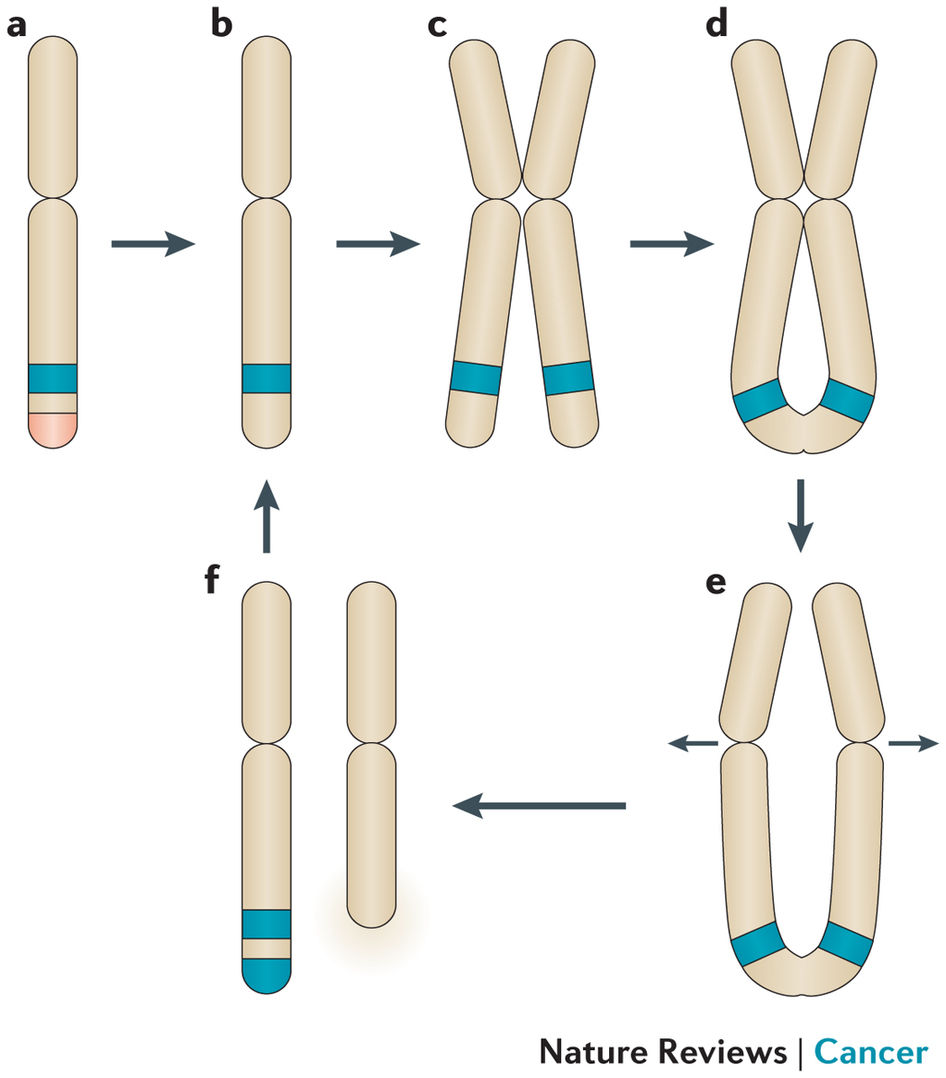
\includegraphics[height=12cm, keepaspectratio]{BFB.jpg}% picture filename
	  \captionsetup{justification=centering,margin=0.5cm, singlelinecheck=off}
	  
	  \caption[]{
	  Schematizzazione del processo BFB (breakage-fusion-bridge) \cite{BFBImage}: 
	  \begin{itemize}
	  \item \textbf{a}: un cromosoma aploide normale, con i telomeri;
	  \item \textbf{b}: perdita del telomero (breakage)
	  \item \textbf{c}: nella formazione del cromosoma diploide due estremità risultano adiacenti e prive di telomeri
	  \item \textbf{d}: i due cromosomi si fondono alle estremità (fusion)
	  \item \textbf{e}: alla successiva duplicazione il cromosoma fuso è tirato alle estremità (bridge)
	  \item \textbf{f}: le cellule figlie mostreranno un insieme di cromosomi asimmetrico, e il processo si ripeterà dal punto b     
	  \end{itemize}} \label{fig:BFB}
	
	\end{figure}

	I tumori mostrano anche delle notevoli differenze da paziente a paziente, fra queste vi è il modo in cui le mutazioni di tipo SNV si accumulano,
	caratteristica che varia notevolmente in funzione del trattamento a cui il malato è sottoposto.
	Infatti, è proprio il \textbf{trattamento} che può causare diversi fenomeni incrementando esso stesso
	il panorama delle mutazioni (ad esempio provocando delle rotture a doppio filamento nell'elica di DNA) oppure al contrario, sopprimendo l'ipermutabilità.
	E' stato spesso assunto che la selezione e la differenziazione delle cellule cancerose sia guidata da un
	processo evolutivo dinamico che le porta ad adattarsi all'ambiente. Altri studi hanno però mostrato come
	queste considerazioni giochino un ruolo secondario nell'evoluzione tumorale, in contrasto con l'evoluzione
	delle specie. Gli elevati livelli di eterogeneità nelle sub-popolazioni colonali portano ad ipotizzare una
	condizione di \textbf{"equilibrio puntuale"} piuttosto che alla competizione per sopravvivenza del più forte; si osserva inoltre che alcuni tumori
	appaiono proprio privi di selezione in mancanza di un trattamento mentre se questo è presente il progresso risulta evolutivo.
	L'\textbf{alta eterogeneità pre-trattamento} gioca un ruolo di rilievo nella adattabilità del tumore, garantendo
	che questo riesca a sopravvivere favorendo la propagazione delle sue sub-popolazioni adatte alla nuova
	condizione (comprovato dal fatto che spesso la progressione alla forma metastatica e la resistenza ai
	farmaci deriva proprio dalle popolazioni poco frequenti nelle fasi iniziali).
	
 	\subsection{\large Le diverse tipologie di studio ed analisi}
		
	Il riconoscimento del ruolo dell'evoluzione nello sviluppo dei tumori ha portato alla formazione
	di un'estensione della filogenetica verso l'analisi del cancro, giungendo alla creazione di un nuovo campo di ricerca chiamato appunto "\textbf{tumor phylogenetics}".
	Dopo i primi passi pionieristici (Tsao \cite{Tsao} con un metodo manuale e Desper \cite{Desper} che per primo ha applicato metodi prettamente filogenetici) lo scopo di
	questa materia è rimasto quello di riuscire a ricostruire l'evoluzione tumorale sfruttando l'informazione
	data dalle variazioni geniche, spesso proprio mediante alberi filogenetici.
	Questi metodi si differenziano per diverse caratteristiche:
	
	\begin{itemize}
	\item \textbf{Design dello studio}: influenza il tipo di dato utilizzato per l'analisi, possono essere svolti su più tumori
	di diversi pazienti, bulk su un singolo paziente o single-cell su un singolo paziente.
	\item \textbf{Tipologia dei dati analizzati}: marker tumorali, come CGH a larga scala (per analizzare CNVs) o FISH
	(fluorecense in situ hybridization), oppure metodi basati sul Next Generation Sequencing per
	l'estrazione di SNVs, CNVs, espressione genica, metilazione o altri marker istonici (modifiche alla
	struttura cromosomica).
	\item \textbf{Modello matematico}: il modello utilizzato incide sull'applicabilità e sull'adesione del metodo filogenetico
	ai dati, per esempio supportando o meno certi tipi di mutazioni come le SVs (structural variants, come
	le CNVs) o assumendo determinati processi evolutivi.
	\item \textbf{Differenze negli algoritmi applicati}: diversi studi sono basati su metodologie che venivano già
	impiegate per la filogenetica delle specie (metodi di massima parsimonia, minima evoluzione,
	neighbour joining, UPGMA (Unweighted Pair Group Method with Arithmetic Mean), massima
	verosimiglianza, inferenza probabilistica bayesiana a volte combinate. Di rado gli algoritmi hanno
	implementazioni che tengono conto delle peculiarità del tumore nella sua evoluzione.
	\end{itemize}

	Gli alberi evolutivi sono centrali in queste ricerche; sono stati impiegati fin dai primi studi che hanno
	provato ad applicare l'analisi filogenetica per trovare le mutazioni guida nel cancro o per ordinarle
	temporalmente, fino a quelli che ora mettono in discussione se l'evoluzione del tumore possa essere
	effettivamente lineare, come nel caso delle specie, o se invece abbia un comportamento ramificato. Il tutto
	nella maggior parte dei casi con lo scopo di predire le traiettorie evolutive del cancro per fini medici.
	
	Il progresso in quest'ambito ha portato ad una grande quantità di software disponibile a questo scopo che si presta facilmente 
	ad un utilizzo erroneo, dando spesso risultati apparentemente discrepanti. Queste inconsistenze sono causate per lo più dalle
	differenze negli studi stessi, ed in particolare dalla tipologia di dati analizzati. Inoltre non vedere una selezione su un 
	qualche tipo di marker tumorale non esclude direttamente la sua totale assenza, dato che questa potrebbe presentarsi in 
	altre caratteristiche non prese in considerazione.   

	\subsection{\large Approfondimento sulle tipologie di studio}

	Si possono distinguere prevalentemente \textbf{tre} metodologie di studio differenti per acquisire i dati necessari all'analisi filogenetica: 

	\begin{itemize}
	\item \textbf{Cross sectional}: (Figura \ref{fig:CrossSectional}) la metodologia più generale, sfrutta dati da \textbf{diversi tumori} provenienti da \textbf{diversi pazienti} per ricostruire i percorsi evolutivi comuni.
	\item \textbf{Regional Bulk}: (Figura \ref{fig:RegionalBulk}) costruisce degli alberi per il \textbf{singolo paziente} prendendo i dati da \textbf{più cellule} provenienti da \textbf{diverse regioni tumorali} o da aree diverse
			              della stessa, valutandone le differenze.
	\item \textbf{Single cell}: (Figura \ref{fig:SingleCell}) la metodologia più precisa e complessa, opera su \textbf{singole cellule} di una \textbf{singola regione tumorale} in un \textbf{singolo paziente}. Di solito in questo caso 
				    sono ripetute diverse acquisizioni dati a diversi tempi per osservare le differenze nel tempo.
	\end{itemize}

	\begin{figure}[H]
	  \centering
	  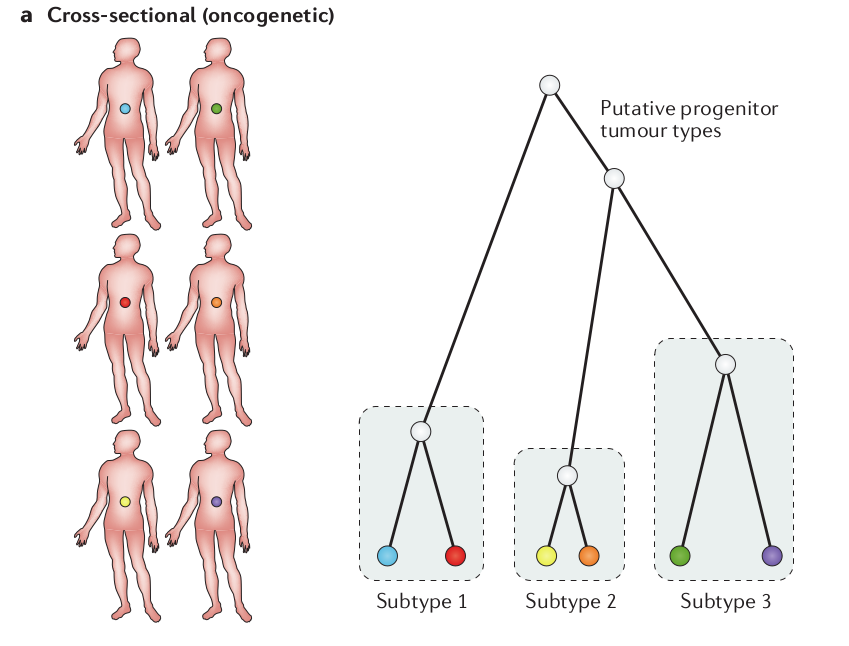
\includegraphics[height=5.5cm, keepaspectratio]{CrossSectional.png}% picture filename
	  \captionsetup{justification=centering,margin=0.5cm}
	  \caption{Modello di studio cross-sectional, dove sono coinvolti diversi pazienti} \label{fig:CrossSectional}
	\end{figure}

	\begin{figure}[H]
	  \centering
	  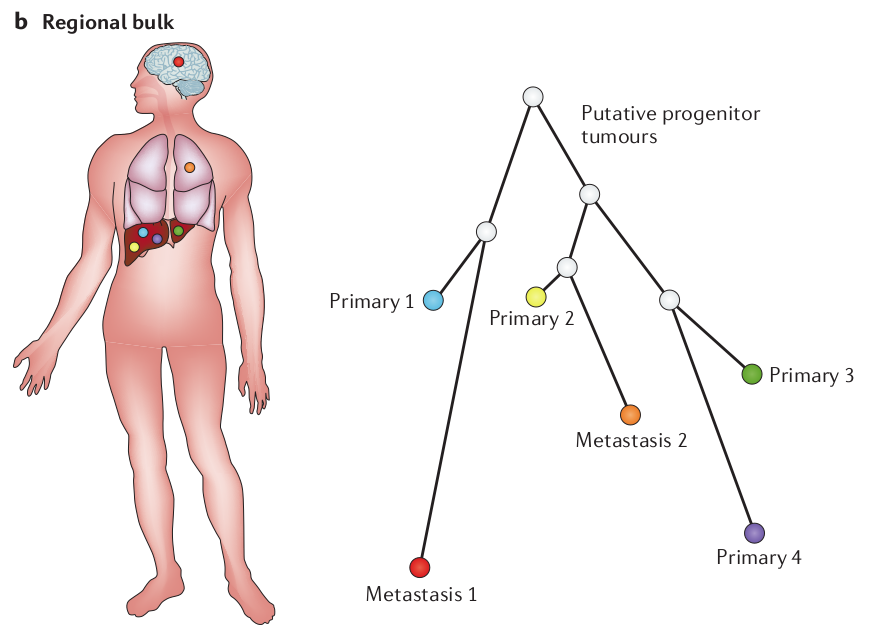
\includegraphics[height=5.5cm, keepaspectratio]{RegionalBulk.png}% picture filename
	  \captionsetup{justification=centering,margin=0.5cm}
	  \caption{Modello di studio regional bulk, dove sono sfruttati dati provenienti da regioni differenti del tumore} \label{fig:RegionalBulk}
	\end{figure}

	\begin{figure}[H]
	  \centering
	  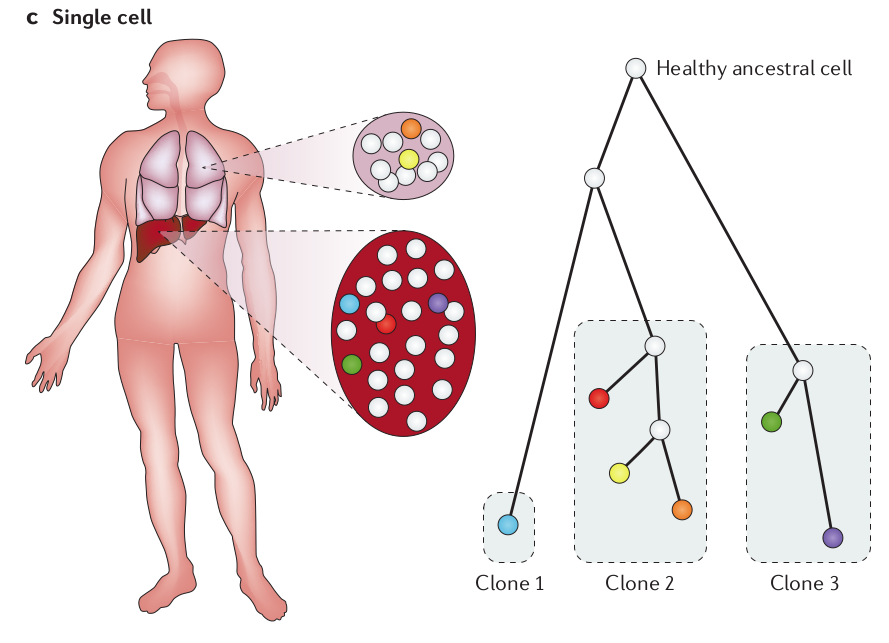
\includegraphics[height=5.5cm, keepaspectratio]{SingleCell.png}% picture filename
	  \captionsetup{justification=centering,margin=0.5cm}
	  \caption{Metodo di studio single cell, ove si analizzano le differenze cellulari fra le singole regioni} \label{fig:SingleCell}
	\end{figure}

	\subsubsection{Modelli per gli studi Cross-sectional}
	
	Il primo modello realizzato per uno studio di carattere filogenetico risale ai lavori di Fearon e Vogelstein \cite{FerVog}, assegnava al tumore un'evoluzione a stadi \textbf{lineare} e veniva preparato 
	manualmente. Il primo esempio di applicazione di metodi filogenetici si deve invece a Desper \cite{Desper} che oltretutto ideò la versione originale degli \textbf{alberi oncogenetici} (alberi i cui nodi sono etichettati da
	geni e gli archi con le probabilità che dalla mutazione del gene sorgente si sviluppi la mutazione sul gene destinatario).

	I primi modelli applicati per la ricostruzione dell'albero erano del tipo \textbf{character based} (i più informativi e complessi algoritmicamente) ossia
	sfruttanti un insieme discreto di marker tumorali basandosi sulla \textbf{massima parsimonia} (i più semplici
	della loro classe, usati da Desper) che ha il difetto di assumere una certa rarità fra le mutazioni, non troppo adatta
	al contesto dei tumori. Seguono poi i metodi \textbf{probabilistici} basati sulla \textbf{massima verosimiglianza} o sul
	\textbf{campionamento bayesiano}, più adatti allo scopo ma più complessi. Approcci più recenti cercano di
	sfruttare al meglio le tecniche moderne di sequenziamento e molti di questi sono basati sul metodo \textbf{MCMC Markov Chain Monte Carlo}, che permette di analizzare un numero maggiore di ricostruzioni
	filogenetiche possibili considerando diversi parametri ma ad un costo computazionale ancora più elevato.
	Un'alternativa sono i metodi \textbf{distance-based} che permettono l'analisi su dataset molto ampi (vengono
	stimate delle distanze fra i samples e cercati i più vicini) sacrificando precisione, il che li rende inadatti in caso di estrema eterogeneità tumorale.
	(Si noti che l'equivalente di massima parsimonia con il metodo distance-based è detto di minima evoluzione, per un riassunto si vedano le tabelle in 
	figura \ref{fig:TabModelli} e \ref{fig:TabAlgoritmi})

	\begin{figure}[h]
	  \centering
	  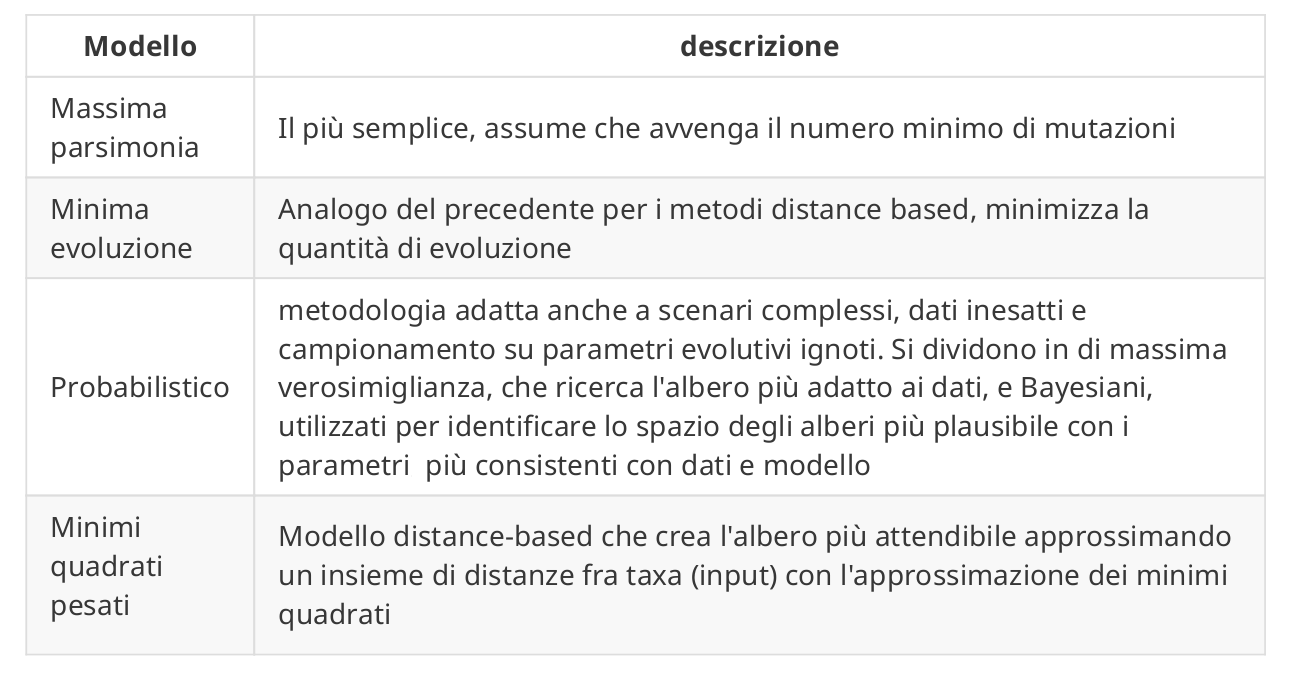
\includegraphics[scale=0.3, keepaspectratio]{TabModelli.png}% picture filename
	  \captionsetup{justification=centering,margin=0.5cm}
	  \caption{I modelli principali usati nell'analisi filogenetica dei tumori} \label{fig:TabModelli}
	\end{figure}

	\begin{figure}[h]
	  \centering
	  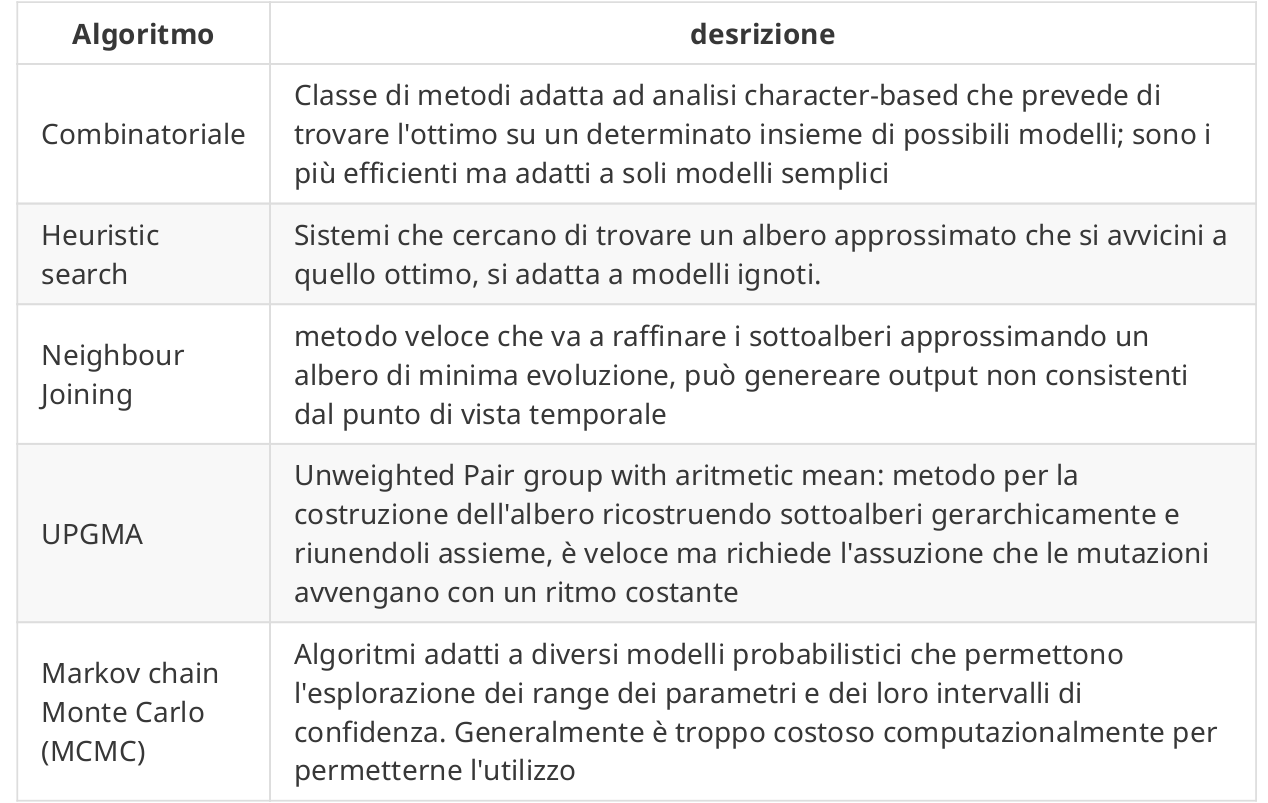
\includegraphics[scale=0.3, keepaspectratio]{TabAlgoritmi.png}% picture filename
	  \captionsetup{justification=centering,margin=0.5cm}
	  \caption{Gli algoritmi principali usati nell'analisi filogenetica dei tumori} \label{fig:TabAlgoritmi}
	\end{figure}

	\subsubsection{Regional Bulk} 
	
	Anche in questo contesto si applicano gli stessi concetti dell'analisi cross-sectional (raramente invece delle euristiche custom), ma spesso sono applicati a metodologie 
	che hanno preceduto l'avvento dell'NGS. Un aspetto importante a questo livello è la \textbf{deconvoluzione dei cloni della sequenza bulk} ossia l'operazione che permette 
	di estrapolare le sub-popolazioni clonali dai dati completi.

	\subsubsection{Single Cell}

	Le prime metodologie applicate per quest'analisi sono state effettuate con sistemi precedenti al
	sequenziamento come FISH o microsatellite markers, ancora utilizzati per la loro capacità di analizzare un
	numero decisamente superiore di cellule. Molti dei sistemi software in questo ambito sfruttano
	sistemi creati per lo studio filogenetico su specie senza sfruttare algoritmi o modelli espliciti.

	\normalsize

	\subsection{\large Un esempio di applicazione pratica}
	Per capire meglio come può essere effettuata un'analisi corretta per un proprio studio con i metodi di
	inferenza filogenetica, l'autore della review propone una simulazione realistica dove evidenzia le molteplici possibilità di
	errore che viene qui riproposta. 

	\begin{itemize}
	\item \textbf{DOMANDA}: quali sono le tempistiche e la sequenza con cui le CNVs si visualizzano nell'evoluzione del
	cancro al seno?
	\item \textbf{DATI}: sequenziamento del DNA su tutto il genoma con copertura di 50x da 200 cellule tumorali con
	genoma normale di riferimento.
	\end{itemize}

	Si assuma inoltre di conoscere la vera storia evolutiva del tumore (si consideri l'immagine \ref{fig:EsNormale} come 
	esemplificativa) 

	\begin{figure}[H]
	  \centering
	  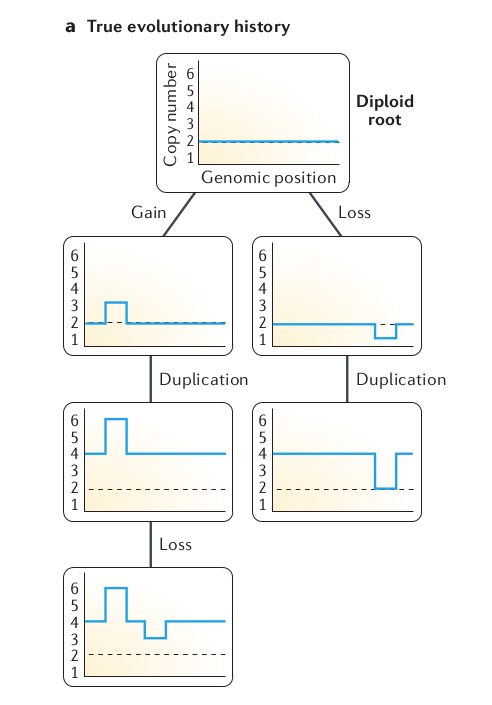
\includegraphics[scale=0.3, keepaspectratio]{EsNormale.png}% picture filename
	  \captionsetup{justification=centering,margin=0.5cm}
	  \caption{La vera storia evolutiva del tumore} \label{fig:EsNormale}
	\end{figure} 

	\subsubsection{Consistenza fra modello e dati}
	
	Sfruttando un programma già pronto basato sul neighbour joining è possibile ottenere un albero
	filogenetico già direttamente, molto simile a quelli degli studi a cui è stato applicato.

	\begin{itemize}
	\item \textbf{PROBLEMA}: Questo può essere dovuto all'approccio impiegato che non è adatto all'analisi delle
	mutazioni di tipo CNV, mentre è nato per quelle SNV, dato che assume che le mutazioni si accumulino \textbf{una
	per volta} con una \textbf{frequenza costante} e un cambiamento di molte basi sarebbe mal interpretato (Figura \ref{fig:EsModello}).
	\item \textbf{SOLUZIONE}: Per riuscire a trattare le CNV si deve utilizzare un modello compatibile, come ad esempio
	quello probabilistico bayesiano che si adatta anche a scenari evolutivi complessi.
	\end{itemize}

	\begin{figure}[H]
	  \centering
	  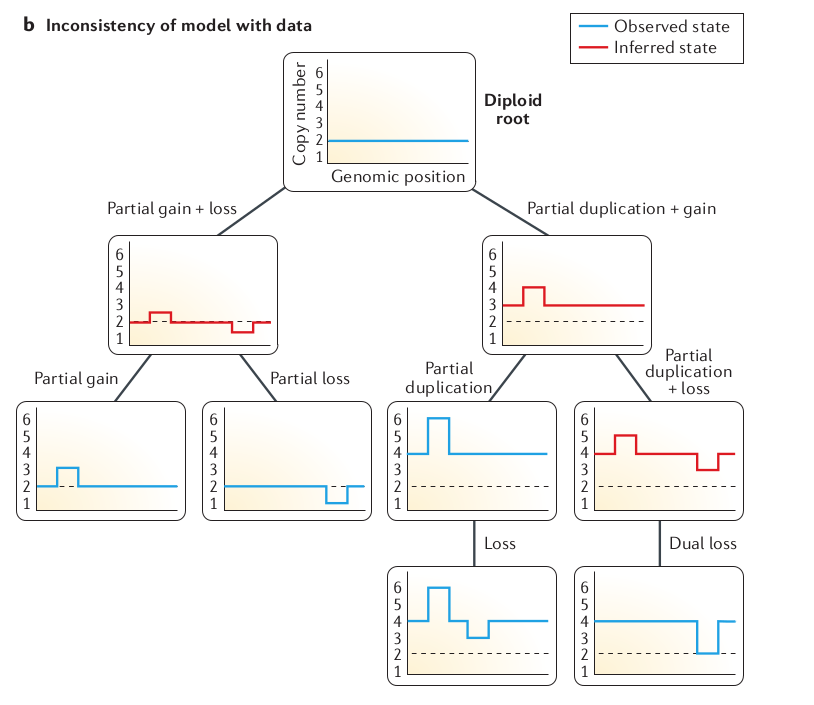
\includegraphics[scale=0.3, keepaspectratio]{EsModello.png}% picture filename
	  \captionsetup{justification=centering,margin=0.5cm}
	  \caption{Risultato dell'inferenza ottenuta tramite neighbour-joining, si può notare come la 
	dimensione delle mutazioni coinvolte venga mal interpretata, producendo dei guadagni o perdite parziali di geni, non 
	realistiche} \label{fig:EsModello}
	\end{figure}

	\subsubsection{Compatibilità algoritmo e modello}

	\begin{itemize}
	\item \textbf{PROBLEMA}: cambiando il modello è necessario cambiare anche l'algoritmo che opera sui dati.

	\item \textbf{SOLUZIONE}: In questo contesto si può scegliere di usare metodi che sfruttino l'MCMC Sampling, che sono
	lo standard per riuscire ad approssimare modelli probabilistici complessi su cui non si ha una teoria
	precisa.
	\end{itemize}

	\subsubsection{Compatibilità fra algoritmo e dati}
        
	\begin{itemize}
	\item \textbf{PROBLEMA}: Ogni algoritmo porta con sè delle limitazioni specifiche ed è necessario che
	queste siano rispettate dai dati. Nel caso di esempio si ha che l'algoritmo MCMC ha la caratteristica di
	avere una complessità esponenziale secondo il numero di cellule, dove in particolare 200 non è una quantità accettabile.
	(Si osservi la figura \ref{fig:EsAlgoritmo})
	\item \textbf{SOLUZIONE}: Queste metodologie sono normalmente adatte solo a decine di specie, dunque una scelta
	possibile è quella di adattare i dati a questo algoritmo, e di passare da un'analisi single cell ad una bulk,
	ove sono sequenziate 10 diverse regioni provenienti da 20 gruppi di cellule tumorali differenti, adattando
	così dati e algoritmo.
	\end{itemize}

	
	\begin{figure}[H]
	  \centering
	  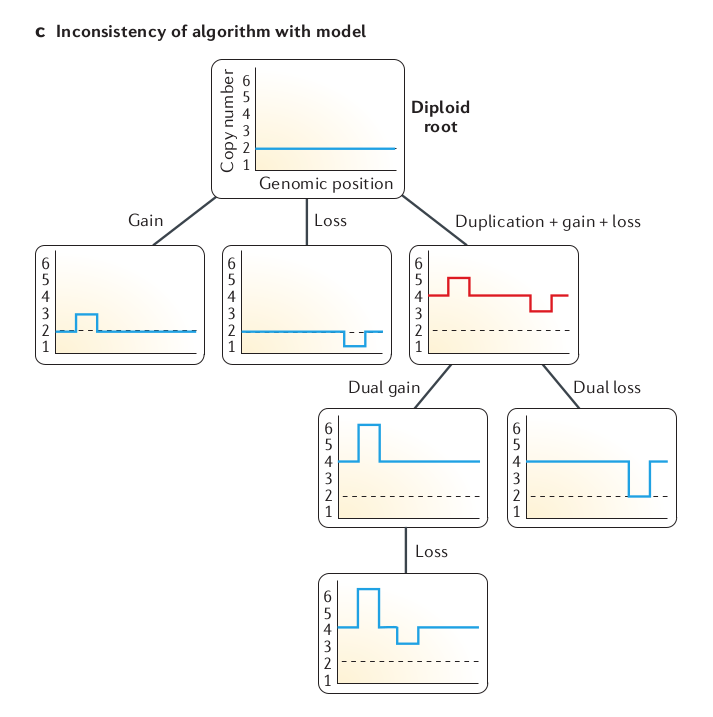
\includegraphics[scale=0.30, keepaspectratio]{EsAlgoritmo.png}% picture filename
	  \captionsetup{justification=centering,margin=0.5cm}
	  \caption{Errore dovuto all'allineamento dati-algoritmo, pur ottenendo un risultato più accurato la complessità elevata 
	delle operazioni non permette di raggiungere l'albero ottimo e questa situazione è dovuta al troncamento dell'esecuzione} \label{fig:EsAlgoritmo}
	\end{figure}

	\subsubsection{Compatibilità fra metodo e domande}
	
	\begin{itemize}
	\item \textbf{PROBLEMA}: Con la soluzione imposta al passo precedente non è possibile avere la risoluzione necessaria
	per poter rispondere alla domanda originale, dato che nelle CNV accade spesso che i tumori mostrino
	difetti di replicazione che portano all'accumulazione di queste mutazioni in sub-cloni che sono rari negli
	stadi iniziali della malattia. (si analizzano troppe poche regioni, ove si possono verificare multiple CNV, come
	esemplificato in figura \ref{fig:EsDomanda})
	\end{itemize}

	\begin{figure}[H]
	  \centering
	  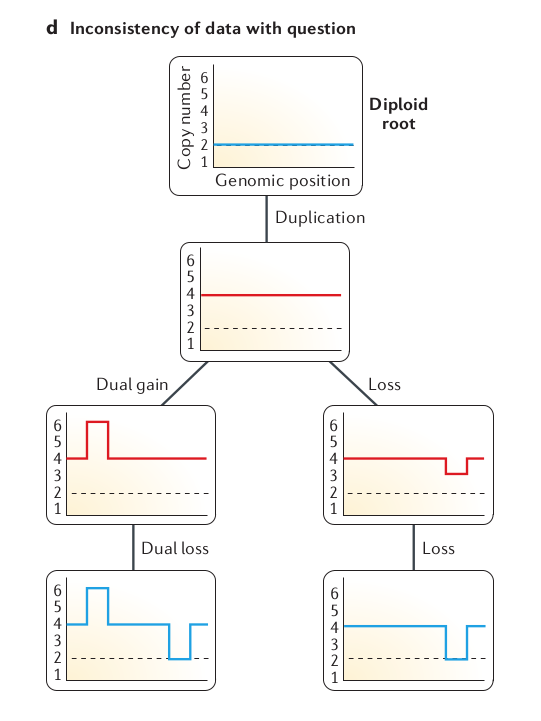
\includegraphics[scale=0.30, keepaspectratio]{EsDomanda.png}% picture filename
	  \captionsetup{justification=centering,margin=0.5cm}
	  \caption{Risultato finale ottenuto dopo aver raggruppato i dati per ridurne l'impatto sulla complessità; non più è possibile 
	distinguere tutti gli stadi evolutivi presenti} \label{fig:EsDomanda}
	\end{figure}

	\subsubsection{Approcci possibili}
	Giunti a questo punto è necessario considerare di rianalizzare a fondo il problema. Una prima
	idea può essere quella di prendere i dati dello studio ed analizzarli con un modello di massima parsimonia,
	più semplice e veloce rispetto a quello probabilistico, una seconda quella di usare algoritmi più esotici ed
	infine una terza quella di sfruttare diverse tipologie di marker (FISH ad esempio).
	In alcune circostanze potrebbe non essere possibile trovare un accordo fra le componenti dello studio
	considerato, a quel punto è necessario riflettere sul fatto che \textbf{non esistono metodi già pronti per molte
	importanti domande} e che potrebbe essere necessario svilupparne uno per la propria (il che richiede competenze
	notevoli in biologia computazionale).

	\section{\LARGE Un software per l'analisi cross-sectional: BML}

	BML (Bayesan Mutation Landscape) è un software recentemente realizzato da Misra et al. \cite{BMLPub} che si propone di sfruttare
	un metodo \textbf{probabilistico} basato sulle reti bayesane per affrontare il problema dell'inferenza dei percorsi evolutivi
	nel cancro. Inizieremo riassumendo il paper realizzato per la pubblicazione di BML per poi discutere invece delle modifiche da 
	me apportate al programma per migliorane la facilità sia d'uso che di modifica.

	\subsection{\large Introduzione}

	Un fenomeno largamente presente in ambito genetico è chiamato \textbf{epistasis} e consiste nell'interazione fra diversi geni,
	che si possono influenzare l'un l'altro favorendosi oppure sfavorendosi vicendevolmente nell'espressione genica. Questo 
	fenomeno è prevalente anche quando le cellule mostrano un comportamento anormale, come accade nei tumori.

	Si può definire \textbf{funzione di benessere} (fitness function, detta anche panorama o landscape) lo spazio di tutti i
	genotipi dipendenti sia dall'importanza che dal comportamento delle interazioni epistatiche fra i geni. I
	genotipi tumorali sono quindi il risultato delle interazioni fra diversi percorsi evolutivi realizzatisi che si distribuiscono
	su un panorama complesso; i pattern che ricorrono fra le mutazioni somatiche contengono informazioni
	su entrambi questi elementi.
	 
	Le metodologie precedenti a BML (2014) che cercano di estrapolare queste informazioni sono tuttavia molto
	complesse computazionalmente e, o non permettono di prendere in considerazione tutti i dati disponibili costringendosi quindi
	a operare su un sottoinsieme degli scenari possibili, o sono utilizzabili esclusivamente su
	piccoli gruppi di geni.

	\subsection{\large L'approccio di BML}

	BML, a differenza di molti altri software, ha la caratteristica di prendere in
	considerazione anche quei \textbf{genotipi ancestrali} sconosciuti (che precedono la condizione attuale del tumore)
	prima di andare ad inferire i \textbf{percorsi di progressione evolutiva (EPP in inglese)}. Gli stadi ancestrali, la cui
	non considerazione spesso è un problema intrinseco a questo tipo di analisi, vengono stimati da BML
	direttamente dai dati. Inoltre, in questo metodo vengono inserite delle \textbf{ottimizzazioni algoritmiche} che
	permettono di calcolare gli EPP anche dei più grandi dataset disponibili considerando tutti i dati (nel 2014).
	
	Come già accennato BML è basato su un modello \textbf{probabilistico} dove ogni percorso evolutivo dal genotipo sano a ognuno di quelli tumorali ha probabilità non nulla. 
	Indichiamo con $P(g)$ la probabilità che un genotipo $g$ sia presente nell'evoluzione del tumore (probabilità evolutiva) e che raggiunga la fissazione.
	Per ogni genotipo questo valore è uguale alla somma di tutti i percorsi evolutivi passanti per lui e che terminano con un genotipo tumorale (Dunque $P(s)=1$ dove $s$ il genotipo sano).
	Si osserva inoltre che $P(g)$ è approssimabile con il valore $n(g)/N$ dove con $n(g)$ indichiamo il numero di campioni che hanno g come stato ancestrale o corrente e con N il numero complessivo dei campioni. 
	In questo modo $P(g)$ è influenzato dal panorama di benessere che si sviluppa attraverso gli stati ancestrali di $g$ attraversati durante l'evoluzione somatica. Questa metodologia inoltre 
	\textbf{assume che le mutazioni si verifichino una per volta} e quindi non è adatta alle mutazioni di tipo strutturale come le CNV, mentre è adatta alle SNV, piccole inserzioni e piccole delezioni.
	Inoltre viene \textbf{ignorato l'effetto delle mutazioni già presenti nella linea germinale}. 

	Questo approccio cerca di stimare la probabilità evolutiva utilizzando un modello basato sulle \textbf{reti bayesiane},
	che possono essere rappresentate con dei grafi orientati e aciclici (DAG). BML stima la probabilità dei percorsi evolutivi $P$ 
	anche per gli stati ancestrali basandosi su probabili percorsi evolutivi illustrati con degli alberi biforcati. 
	I nodi interni di questi alberi rappresentano i genotipi ancestrali e assieme a quelli tumorali vengono usati per il learning della rete bayesiana. 
	Dato che i percorsi evolutivi non sono noti è necessario operarare sugli alberi e in questo caso è stato scelto il metodo chiamato  \textbf{nearest nighbour interchange} 
	(NNI) che permette così il computo di un \textbf{ottimo locale} a partire da un albero casuale. La rete bayesiana successivamente stimerà $P$ (tranne che per un fattore di normalizzazione,
	che successivamente sarà impostato proprio per avere $P(s)=1$ con $s$ il genotipo normale) e questa stima verrà usata per calcolare i percorsi di progressione evolutiva più probabili
	e successivamente visualizzarli. Inoltre sarà possibile osservare la distinzione fra \textbf{interazioni epistatiche positive dirette e indirette} (le negative non sono considerate) 
	dove quelle dirette saranno indicate da archi nella rete.

	Si osservi l'immagine \ref{fig:SchemaBML} per avere una panoramica degli stadi di elaborazione di BML.

	\begin{figure}[h]
	  \centering
	  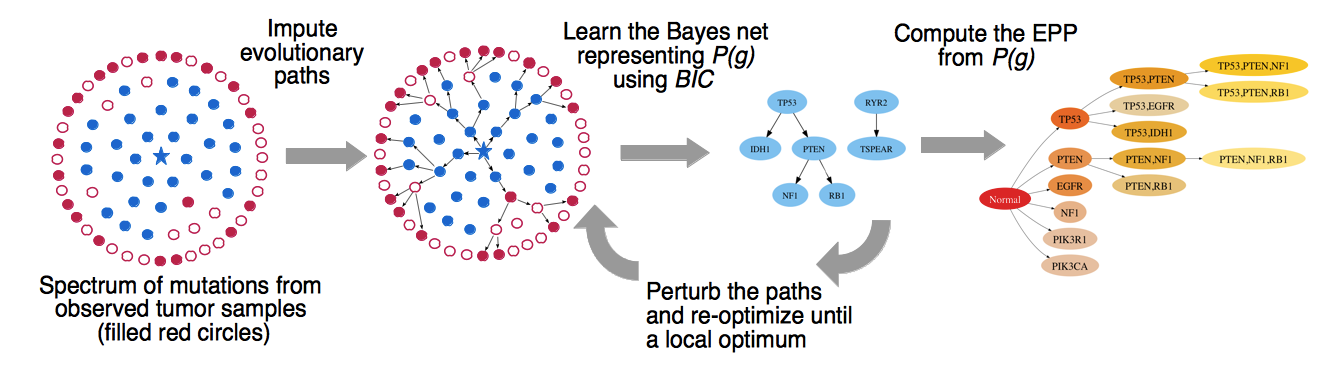
\includegraphics[scale=0.13, keepaspectratio]{SchemaBML.png}% picture filename
	  \captionsetup{justification=centering,margin=0.5cm}
	  \caption{Questo schema illustra il processo di inferenza di BML (mostrato per il Glioblastoma). Nella prima immagine a destra è possibile
	  vedere la presentazione dell'assetto reale delle mutazioni, con pallini rossi per gli stadi tumorali (pieni se osservati) e blu per 
	  gli stadi ancestrali, con una stella per il genotipo normale. Nella seconda si osserva la ricostruzione degli alberi evolutivi radicati nel
	  genotipo normale usati, come si vede nella terza immagine, per ottenere la rete bayesiana.
	  Infine viene mostrato il grafo di output corrispondente ai percorsi evolutivi tumorali ottenuti dalla rete} \label{fig:SchemaBML}
	\end{figure}

	\subsection{\large Learning della rete bayesiana e ricostruzione degli EPP}

	\subsubsection{I dati}

	I dataset su cui BML è stato testato sono diversi, disponibili pubblicamente e toccano diversi tipi di cancro, come quello del colon retto,
	il glioblastoma, quello ai polmoni, alle ovaie e al seno. I dati sono stati preprocessati prima dell'analisi 
	per fare in modo di rimuovere samples anormali, selezionare solo i geni più mutati (tramite una soglia) e di considerare solo le mutazioni compatibili con questo metodo.
	Da queste informazioni viene estratta una matrice mutazioni/campioni che ha in ogni posizione un 1 se il gene nel dato sample è mutato e 0 altrimenti. 
	BML è inoltre compatibile con programmi esterni di selezione delle mutazioni per poter operare sotto criteri differenti.
	In assenza di informazioni funzionali, l'output di questo programma va letto in soli termini probabilistici, senza assegnare ruoli specifici ai percorsi evolutivi mostrati.

	\subsubsection{Il modello} 

	Una \textbf{rete bayesiana} $B(G, \Theta)$ è definita da $G$ un grafo orientato e aciclico (DAG) i cui vertici ($V$) sono variabili booleane aleatorie
	e $\Theta = \{\theta_{C}|C\in V\}$ un insieme di parametri che rappresentano le probabilità condizionali $Pr(C=c|\Pi_{C}=\pi)\equiv \theta_{C}(c|\pi)$,
 	ove $c$ è lo stato di una variabile e $\pi$ il relativo stato dei suoi genitori (fra tutti gli stati dei genitori dei vari nodi, $\Pi_{C}$) in $G$. 
	Si consideri quindi $D$ la matrice di input descritta nella sezione "I dati" e sia $V$ 
	(della rete) l'insieme dei geni e $S$ l'inseme dei campioni. La matrice può essere utilizzata per acquisire
	un numero di dati sufficiente al learning della rete effettuando conteggi del tipo $n_{c,\pi}$ dove sono contati
	il numero di campioni in cui $C=c$ e $\Pi=\pi$.

	Per selezionare le strutture adatte alla rete viene usato il \textbf{BIC} (Bayesan Information Criterion):	

	$$log Pr(D|B) = \sum_{C \in V}Fam(C, \Pi_{C})$$

	dove $Fam(C, \Pi_{C})$ è il punteggio BIC per la famiglia $\{C, \Pi_{C}\}$ (geni e stato dei relativi genitori) che è dato da:

	$$Fam(C, \Pi_{c}) = max_{(\theta_{c})}(\sum_{\pi \in \Pi_{c}}(\sum_{c\in C}(n_{c,\pi}log[\theta_{C}(c|\pi)] -log(n)/2))) $$

	Dal quale, tramite massimizzazione, è possibile, con un numero sufficiente di campioni da una rete bayesiana reale, ricostruirla. 

	\subsubsection{Apprendere le distribuzioni di probabilità}

	Come già detto, per calcolare $P$ è necessario considerare un dataset contenente sia i genotipi tumorali che quelli ancestrali.
 	Per riuscire ad ottenere questi ultimi vengono costruiti degli alberi biforcati con il genotipo normale alla radice, i genotipi tumorali 
	come foglie e i nodi interni con un genitore e esattamente due figli, che vengono poi usati per il learning della rete. 
	Si consideri ogni nodo come una sequenza di valori booleani (1 mutato, 0 non mutato) che, essendo associati ordinatamente a ogni gene, rappresentano il genotipo di una data sub-popolazione tumorale o ancestrale;
	la radice è quindi una sequenza di soli zeri.

	\subsubsection{Semplificazioni e assunzioni}

	\begin{enumerate}
	\item Le mutazioni sono \textbf{irreversibili} ossia se vi è una mutazione in un gene di un nodo, allora questa comparirà in tutti i suoi discendenti
	\item La probabilità degli stati mutati deve essere più piccola di quella dello stato normale (deriva dal modello utilizzato, è implementata facendo in modo che il numero
	di samples che presentano una mutazione su qualche gene non superi la metà del numero di samples analizzati)
	\item Si fa in modo che, dato un genotipo, la probabilità di accumulare una mutazione in un gene non aumenti perdendo una mutazione in un altro gene. Ossia che 
	$$Pr(C=1|\Pi_{C}=\pi_a)\ge Pr(C=1|\Pi_{C} =\pi_b)\forall (\pi_b | \pi_b\subset \pi_a)$$
	con $\pi_b \subset \pi_a$ che va inteso indicando che tutte le mutazioni presenti in $\pi_b$ sono presenti anche in $\pi_a$
	\end{enumerate}

	A questo punto l'\textbf{obiettivo} nel learning della struttura è dato dal trovare $T_*$ albero e $B_*$ rete bayesiana, che massimizzano la BIC score: 
	$$(T_*,B_*) = arg \max_{T,B}{log(Pr(D|B))}$$
	con $D = T \cup O$ dove $O$ sono i genotipi della matrice passata in input.

	\subsubsection{Algoritmo di learning dei parametri della rete bayesiana}

	Dato un albero realizzato come sopra si ricerca la struttura ottimale della rete (DAG) tramite una metodologia detta \textbf{ordering-based search} (OBS)
	che inizializza un ordinamento delle variabili e obbliga ognuna di queste a scegliere i propri genitori esclusivamente dai precedenti nell'ordine. 
	L'algoritmo successivamente ricerca nello spazio di tutti gli ordinamenti invertendo l'ordine di ogni coppia adiacente 
	(per la ricerca nello spazio degli alberi viene usato il set di operazioni NNI).

	\subsubsection{Ricostruzione dei EPP più probabili}  

	Gli EPP sono ricostruiti basandosi sul fatto che gli antenati più probabili per un dato genotipo sono quelli con la più alta probabilità evolutiva.
	L'algoritmo procede considerando tutti gli stati con $k$ mutazioni e ricostruisce la loro storia evolutiva collegando ogni genotipo al suo più probabile stato ancestrale secondo $P$.
	L'input è costituito da tre parametri ossia $P$, $k$ e $c$ dove $0<c<1$ rappresenta un parametro per una soglia che fa in modo di permettere la visualizzazione dei soli nodi
	(con $x$ mutazioni) con probabilità superiore a $c*m_{x}$ dove $m_x$ rappresenta la probabilità massima ottenuta considerando genotipi con $x$ mutazioni ($x\le k$).  
	L'algoritmo itera partendo da $x=k$ e termina quando $x=0$ decrementando $x$ di 1 ad ogni passo.
	(si noti che $k$ è fissato a 3 al momento)

	\subsubsection{Fitness epistasis e la sequenza delle mutazioni}  

	Le interazioni epistatiche contribuiscono sia alla distribuzione delle mutazioni nello spazio dei genotipi e sia alla probabilità evolutiva. \textbf{BML non segue alcun modello specifico} per le dinamiche evolutive. In ogni caso si sfruttano queste due definizioni nell'analisi:
	\begin{enumerate}	
	\item \textbf{fitness epistasis positiva}: intesa come la maggior probabilità che due mutazioni $A$ e $B$ occorrano assieme anzichè separatamente ($P(AB) \ge P(A)P(B)$).
	\item \textbf{sign epistasis}: si ha che $P(A)>>P(B)$ ma, se $A$ occorre con frequenza sufficiente e l'interazione epistatica è sufficientemente forte si ha che $P(A)\le P(AB) \le P(B)$
	(ossia una mutazione che da sola non ha successo, lo ha se si trova assieme ad un'altra mutazione positiva)
	\end{enumerate}

	In BML si sfrutta la stima di $P$ per osservare quando il genotipo doppiamente mutante ha una probabilità evolutiva fra quella dei singoli mutanti,
	dato che questa condizione permette di dare un ordinamento univoco alla relazione di epistasis fra i geni considerati.

	\subsubsection{Procedure di bootstrap}  

	Il bootstrap parametrico richiede di effettuare il learning del modello e di simularlo al fine di generare nuovi dataset permettendo 
	di stimare accuratezza e robustezza dell'algoritmo di learning stesso. I campioni di bootstrap sono ottenuti simulando la rete bayesiana calcolata precedentemente 
	e selezionandone solamente quelli che mostrano almeno una mutazione e dove tutte le mutazioni presenti sono quelle rilevate in almeno uno dei genotipi osservati.

	%--------------------------------- Presentazione del lavoro

	\section{\LARGE Guida e apporti personali a BML}

	\subsection{\large Apporti personali}

	Per quanto il software BML fosse funzionante mancavano alcuni dettagli per la sua completezza. La maggior parte del lavoro è stata di ristrutturazione
	del codice, aggiungendo diversi commenti, correggendo dei bug minori e migliorando l'efficienza di alcune delle sue componenti. Inoltre sono state introdotte
	alcune nuove funzionalità:

	\begin{itemize}
 	\item Un \textbf{preprocessor} per eseguire l'analisi direttamente dai file MAF (Multiple Annotation Format) \cite{MAF} disponibili nei pacchetti dati 
	dei vari studi. Permette inoltre di selezionare le tipologie di mutazioni e i geni che devono essere sfruttati per l'analisi.
	\item Funzionalità di \textbf{multithreading} che permettono di parallelizzare le analisi su diversi alberi (per la ricerca dell'ottimo globale) 
	      e l'analisi dei diversi campioni di bootstrap. L'incremento prestazionale osservato è pari al numero di core disponibili sulla macchina.
	\item Un'\textbf{interfaccia grafica}, che permette di effettuare l'analisi in modo semplice, tramite pochi passi.   	
	\item Un \textbf{sistema di aiuto}, che permette all'utente di accedere rapidamente a una guida rapida, al download dei dati degli studi sul cancro da cBioPortal e 
	alle pubblicazioni riguardanti BML \cite{BMLPub, cBio, BMLSite}. Se invece si volesse 
	scaricare il software originale è possibile farlo da qui \cite{BMLSite} in particolare dalla sezione "Download BML".	

	\end{itemize}
		

	\subsection{\large Guida}

	Nota: al momento il software realizzato ancora non è disponibile online e lo sarà il prima possibile, perciò questa sezione non è completa.

	Per presentare al meglio il software nella sua interezza viene proposta qui di seguito una \textbf{guida completa} al suo utilizzo. E' possibile scaricare
	il codice sorgente di questo programma dal sito ... (TODO sito in allestimento), nella versione da compilare con i sorgenti, (TODO requisiti, guida compilazione)
	oppure precompilata per Windows (a 32-bit) o Linux (a 64-bit) (TODO link prima di QT nelle citazioni). Il programma è stato realizzato utilizzando
	il linguaggio C++ e per l'interfaccia grafica è stata usata la libreria portabile Qt \cite{Qt} in particolare la versione 5.9.1 per Linux e la 
	5.8.3 (TODO) per Windows (compilata con VS2013, elemento fondamentale).

	Il programma è stato testato su due macchine distinte con Ubuntu 16.04 LTS e Windows 10 (in dual boot su entrambe) utilizzanti una 
	un Intel Core i5-2520M CPU a 2.50GHz (2c/4t) e 8GB di RAM e l'altra un Intel Core i7-4820K CPU a 3.70GHz (4c/8t) e 16 GB di RAM.

	\subsubsection{Compilazione ed esecuzione}
	
	Per eseguire il programma sfruttando i pacchetti precompilati è necessario decomprimere gli archivi scaricati (formato .zip)
	e lanciare direttamente l'applicazione BML\_GUI.exe se si usa Windows, oppure eseguire AppRun
	se si usa Linux (che si occupa del caricamento corretto delle librerie).
	Per compilarlo direttamente ... (TODO)

	\subsubsection{Interfaccia primaria}
	
	La finestra principale di BML (figura \ref{fig:BMLMainMenu}) si presenta come un modulo da compilare
	e si occupa di richiedere ed acquisire i dati necessari per l'analisi 
	all'utente. 

	\begin{figure}[H]
	  \centering
	  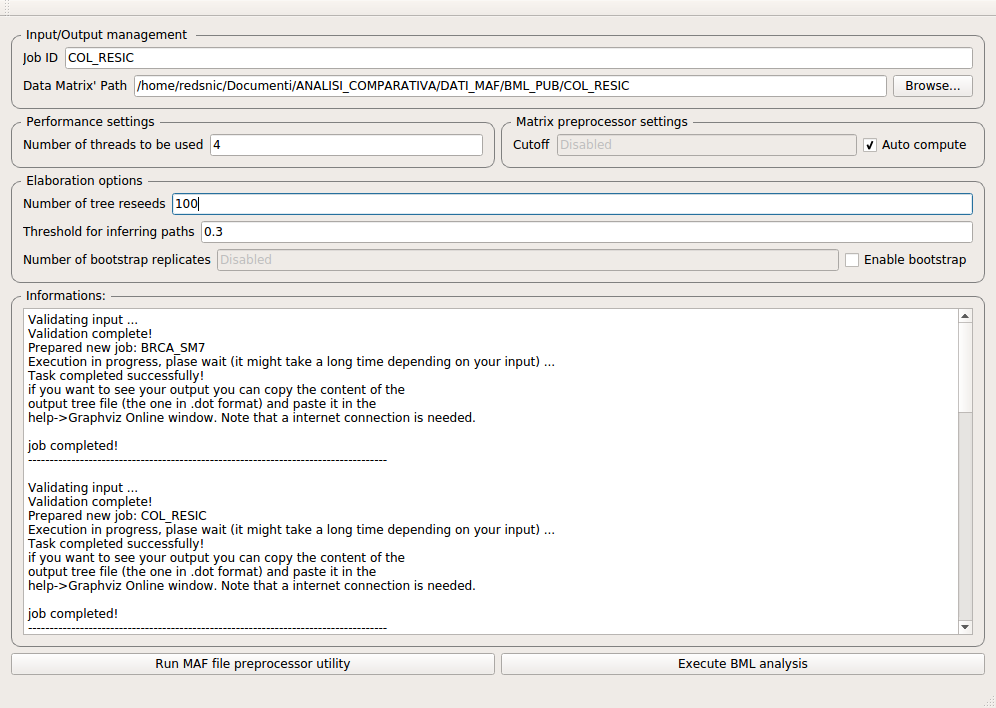
\includegraphics[scale=0.36, keepaspectratio]{BMLMainMenu.png}% picture filename
	  \captionsetup{justification=centering,margin=0.5cm}
	  \caption{La pagina principale della GUI di BML impostata per l'analisi del cancro al colon retto} \label{fig:BMLMainMenu}
	\end{figure}

	Per rendere l'interazione più semplice l'interfaccia è stata 
	suddivisa in diversi blocchi con un ruolo specifico:
	\begin{itemize}
	\item \textbf{Gestione dell'Input/Output}: in questa sezione è richiesto
	un identificativo per l'analisi da effettuare e la matrice delle mutazioni
	da usare come input per il programma. Si noti che tutto l'output generato
	da BML relativo all'analisi corrente conterrà nel nome l'ID scelto dall'utente 
	e sarà posizionato nella cartella 'output' nella stessa directory in cui 
	si trova l'eseguibile (se questa non presente, verrà creata). Inoltre
	I file con lo stesso nome (quindi con lo stesso ID) verranno automaticamente
	riscritti. Si raccomanda inoltre di utilizzare ID che siano accettabili
	come nomi di file nel sistema in uso. 
	\item \textbf{Impostazioni di performance}: da qui è possibile
	selezionare il numero di thread da sfruttare per l'analisi. Di default è 
	utilizzato esattamente il numero di processori logici
	disponibili sulla macchina in uso (per cui il valore ottimale).
	E' possibile diminuire il numero di thread usati per ridurre 
	il carico sulla	CPU al prezzo di performance minori. 
	\item \textbf{Preprocessor della matrice delle mutazioni}: questa opzione
	permette di impostare il numero minimo di volte che una mutazione su un
	particolare gene si debba  
	verificare nei vari campioni affinchè il gene relativo venga considerato
	nell'analisi.
	Spuntando la casella 'Auto compute' questo valore verrà calcolato 
	automaticamente e impostato alla minima soglia che 
	fa sì che il numero di geni sia inferiore al numero di campioni.  
	(Si ha inoltre intenzione di introdurre un secondo parametro in questa sezione 
	che permetta all'utente di effettuare l'analisi al più sugli $N$ geni più mutati, permettendo 
	un controllo più intuitivo sulla quantità di geni coinvolti nell'analisi) 
	\item \textbf{Opzioni di elaborazione}: qui sono raccolti i parametri necessari a BML per
	l'esecuzione dell'analisi:
	\begin{enumerate}
	\item \textbf{Numero di alberi randomizzati da generare}: richiede all'utente il numero 
	di alberi casuali da utilizzare come punto di partenza per l'inferenza della struttura della rete bayesiana
	(più è alto più ci si può avvicinare all'ottimo globale). Questo parametro ha un impatto rilevante sul tempo
	di esecuzione che (tralasciando l'analisi di bootstrap) può essere approssimato tramite la seguente formula
	empirica: 

	$$T_{exe} = \max(\frac{T_{single}}{N_{cores}} * N_{reseeds}, T_{single})$$ 

	ove $T_{single}$ è il tempo di esecuzione medio 
	dell'analisi di un albero, $N_{cores}$ il numero di core fisici utilizzati (i core logici incidono 
	molto meno) ed infine $N_{reseeds}$ il parametro qui inserito. Gli autori di BML avevano impiegato per 
	i loro scopi un valore di 100 o 1000 per questo parametro.    	
	
	\item \textbf{Soglia per l'inferenza dei percorsi (evolutivi)}: Questo parametro è gia stato citato in 
	precedenza con il nome $c$ (ricostruzione degli EPP più probabili) ed è necessario per
	indicare la minima probabilità affinchè una tripletta, una coppia o un singolo gene vengano 
	rappresentate nel grafo finale dei percorsi evolutivi (rispetto a un valore normalizzato secondo 
	la massima probabilità assoluta ottenuta da una tripletta, una coppia o un singolo gene rispettivamente).
	Nonostante il valore utilizzato dai realizzatori di BML sia 0.3, l'utente può variarlo con lo scopo di 
	creare grafi più o meno ricchi di nodi.   

	\item \textbf{Numero di campioni di bootstrap}: Se l'analisi di bootstrap viene abilitata (ossia spuntando la
	checkbox 'Enable bootstrap') è possibile selezionare il numero di replicati da creare e analizzare
	(anche in parallelo), al fine di ottenere gli intervalli
	di confidenza sugli archi inferiti da BML.
	\end{enumerate}
	\item \textbf{Informazioni}: questa area di testo mostra all'utente delle informazioni utili sulle analisi 
	effettuate e fornisce dei consigli se tutti i dati non sono stati inseriti correttamente.
	\end{itemize} 

	Per lanciare l'analisi, una volta preparati i campi, è necessario premere il pulsante 'Execute
	BML analysis', una volta premuto questo si disabiliterà finchè l'operazione non è completa (nel frattempo è 
	comunque possibile operare sul resto dell'interfaccia liberamente). Quando l'esecuzione sarà terminata 
	verrà aperta una finestra che mostrerà la cartella 'output' per accedere rapidamente ai file generati.
	Dalla pagina principale è inoltre possibile accedere al menù a tendina 'help' e al preprocessore per i file 
	MAF premendo sull'apposito bottone. 
	
	\subsubsection{Il menù di help}	
	
	Il menù di help (figura \ref{fig:BMLHelp}) contiene diverse voci atte sia a fornire all'utente una breve guida sul software, sia a
	fornirgli il rapido accesso a siti web utili.

	\begin{figure}[h]
	  \centering
	  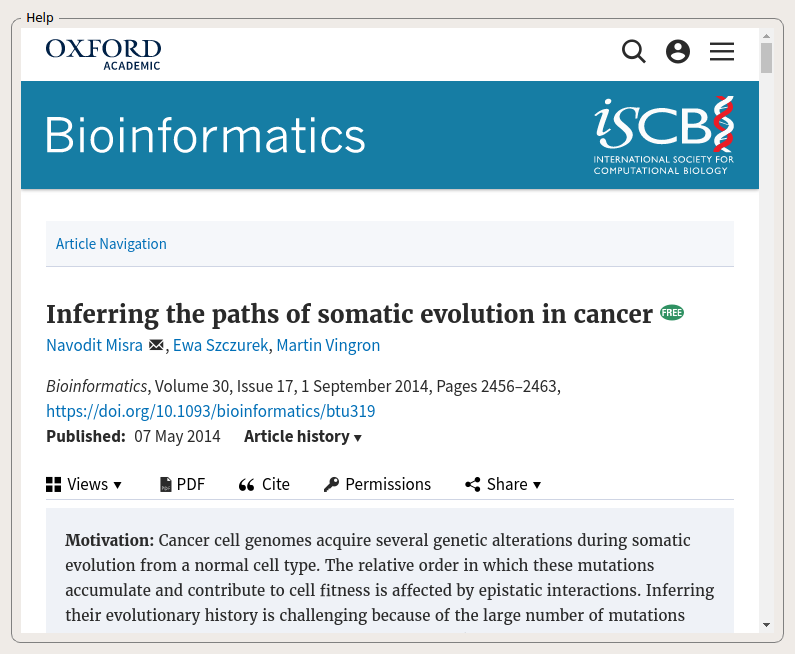
\includegraphics[scale=0.43, keepaspectratio]{BMLHelp.png}% picture filename
	  \captionsetup{justification=centering,margin=0.5cm}
	  \caption{La pubblicazione di BML come viene visualizzata nell'Help} \label{fig:BMLHelp}
	\end{figure}

	Sono elencati qui di seguito:
	\begin{itemize}
	\item \textbf{Guida}: Una guida rapida all'utilizzo di BML e sul significato dei vari parametri. Disponibile
	anche offline.
	\item \textbf{Changelog}: Elenco dei cambiamenti rispetto alla versione originale (eventualmente per 
	versioni successive). Disponibile anche offline.
	\item \textbf{Informazioni su BML}: mostra il sito principale relativo alla versione originale di BML
	\item \textbf{Pubblicazione di BML}: mostra la pubblicazione completa di BML, contiene link ai dati supplementari
	\item \textbf{dataset da cBioPortal}: collegamento alla pagina per scaricare i dataset degli studi sul cancro da
	cBioPortal. 
	\item \textbf{Graphviz Online}: permette l'uso online di Graphviz, il programma necessario per la 
	visualizzazione del grafo creato da BML. E' sufficiente copiare il contenuto dei file .dot
	generati da BML sulla metà sinistra della pagina (uno per volta).
	\end{itemize}

	Si noti che per gli ultimi quattro punti è necessaria una connessione a internet.  

	\subsubsection{Il preprocessore MAF}

	Anche questa utility (figura \ref{fig:BMLMAFPreprocessor}) è stata realizzata con lo stesso criterio della finestra principale. 

	\begin{figure}[h]
	  \centering
	  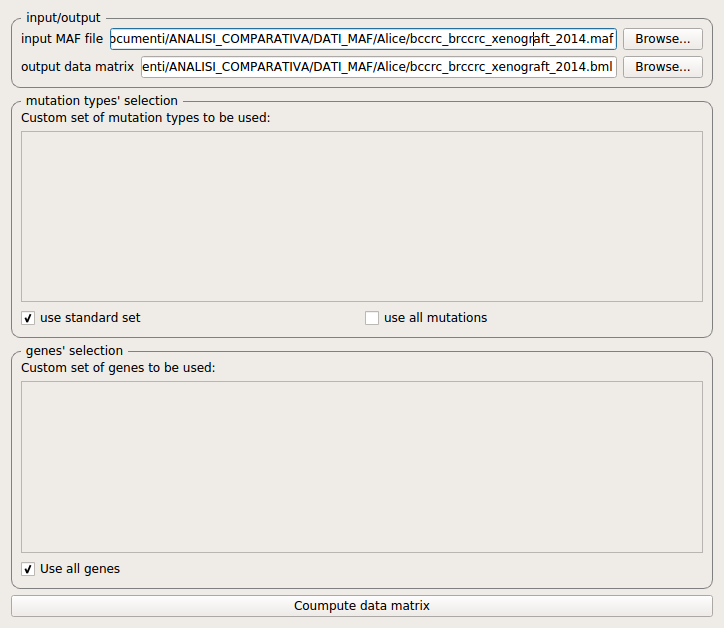
\includegraphics[scale=0.43, keepaspectratio]{BMLMAFPreprocessor.png}% picture filename
	  \captionsetup{justification=centering,margin=0.5cm}
	  \caption{Il preprocessore di file MAF per la traduzione in "mutational array", configurato per operare con le tipologie di
	mutazioni adatte a BML e tutti i geni disponibili } \label{fig:BMLMAFPreprocessor}
	\end{figure}

	E' suddivisa in tre diverse sezioni: 

	\begin{itemize}
	\item \textbf{Input/output}: come dice il nome, vanno inserite le informazioni sull'input (file MAF) e
	sull'output (matrice delle mutazioni per BML). 
	\item \textbf{Selezione dei tipi di mutazione}: Permette di selezionare le tipologie di mutazioni da utilizzare
	durante l'analisi. Vi sono tre modalità:
	\begin{enumerate}
	\item \textbf{Use all mutations}: selezionando la spunta relativa è possibile eseguire BML senza fare distinzioni fra 
	i tipi di mutazione. Questo approccio è sconsigliato dato che questo software non è compatibile con le SVs.
	\item \textbf{Use standard set}: default, usa l'insieme delle mutazioni compatibili con BML, come da pubblicazione.
	\item \textbf{Custom}: Deselezionando entrambe le spunte è possibile inserire manualmente nell'area di testo
	 le tipologie di mutazioni da usare nell'analisi. Si presti attenzione a scrivere gli identificativi correttamente
	 anche per quanto riguarda maiuscole e minuscole.  
	\end{enumerate}
	\item \textbf{Selezione dei geni}: permette di selezionare i geni da sfruttare per l'analisi; è possibile
	usarli tutti (se 'Use all genes' è spuntata) oppure sceglierne un insieme a scelta (se invece non è spuntata) 
	inserendone i codici manualmente. I campioni che non presentano alcuna mutazione nell'inseme di geni scelti verranno
	eliminati dalla matrice generata.  
	\end{itemize}

	Per creare la matrice delle mutazioni a partire dal MAF indicato è sufficiente premere il pulsante
	'compute data matrix'. Un popup comunicherà all'utente l'esito dell'operazione e, in caso di errore, darà 
	delle informazioni su cosa correggere. 

	\section{\LARGE Confronto tra BML e CAPRI}

	In questa sezione confronteremo i risultati ottenuti da BML con quelli di un altra metodologia chiamata CAPRI \cite{CAPRI} facente 
	parte del pacchetto R TRONCO \cite{TRONCO}. 

	\subsection{\large CAPRI: aspetti fondamentali}	

	CAPRI è un metodo probabilistico accoppiato a bootstrap e massima verosimiglianza che si propone di realizzare dei 
	grafi (in particolare dei DAG) ove i nodi sono i geni e gli archi rappresentano la relazione di selezione fra geni
	(con probabilità associata); è possibile vederne uno schema in figura \ref{fig:CAPRI}.

	\begin{figure}[h]
	  \centering
	  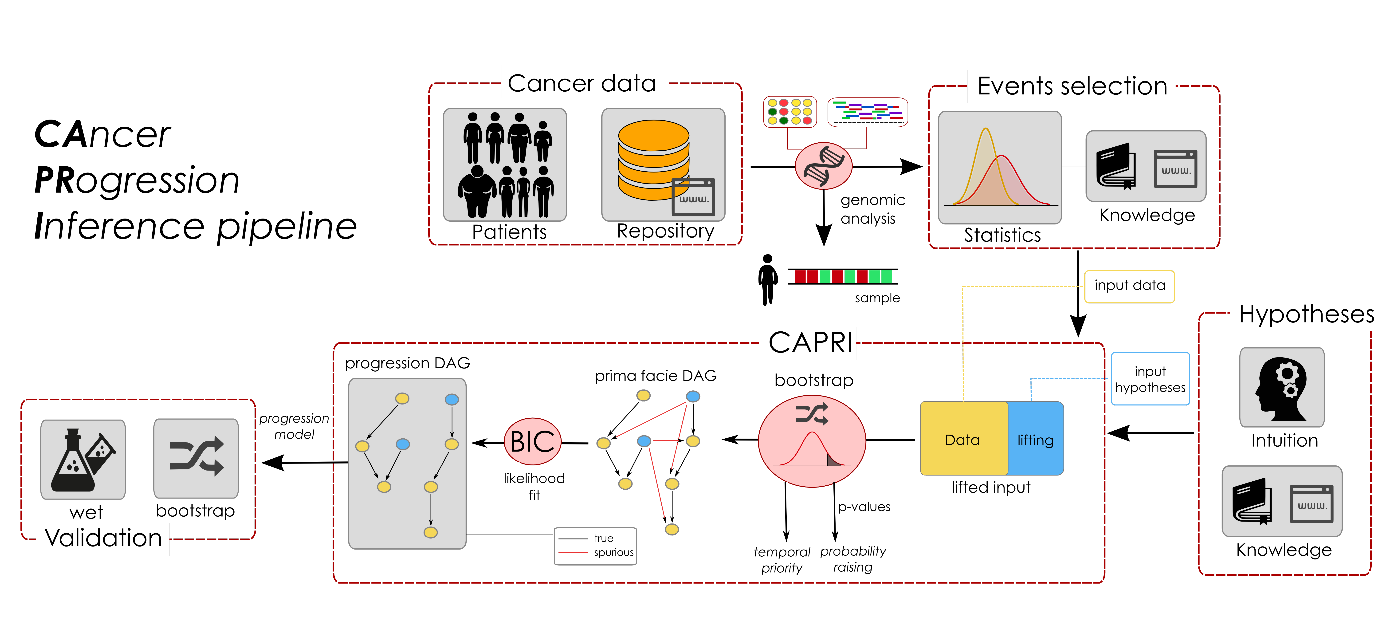
\includegraphics[height=6.7cm, keepaspectratio]{CAPRI.png}% picture filename
	  \captionsetup{justification=centering,margin=0.5cm}
	  \caption{Questo schema illustra come CAPRI si posizioni nell'ambiente della ricerca sul cancro, evidenziando come  
		sia in grado non solo di interfacciarsi ai dati ottenuti, ma anche di integrare la conoscenza pregressa degli esperti} \label{fig:CAPRI}
	\end{figure}

	Questa metodologia viene inoltre presentata come particolarmente efficiente in caso di dati rumorosi, tipici
	degli studi in ambito biologico, ed in particolare con pochi campioni da analizzare. 
	Le relazioni imposte da CAPRI vengono valutate e successivamente raffinate tramite un algoritmo ibrido che 
	ragiona sul tempo, i meccanismi e la probabilità. In particolare la struttura si basa sulla condizione di causa probabilistica di 
	Suppes combinata con fit di massima verosimiglianza e per le probabilità si sfruttano procedure di bootstrap.
	Il risultato ottenuto è un modello basato su un grafo che permette di visualizzare diversi aspetti dell'evoluzione
	del cancro, mostrando ramificazioni, confluenze e progressioni indipendenti.	

	La nozione di \textbf{causa probabilistica} di Suppes può essere così espressa: una relazione di selettività fra due eventi osservabili
	($i$ e $j$) vi è se $i$ precede $j$ dal unto di vista temporale e se la probabilità di osservare $j$ aumenta se condizionata a $i$:
	
	$$P(j|i)>P(j|\lnot i)$$ 

	Il risultato ottenuto a questo punto ha un \textbf{ruolo solo probabilistico} e non prende in considerazione alcuna relazione causa-effetto fra $i$ e $j$.

	La priorità temporale (diciamo di $i$ rispetto a $j$) viene quindi espressa mediante due condizioni:

	\begin{enumerate}
	\item $P(i)>P(j)$ che assume l'accumulazione di eventi (difficilmente le mutazioni sono reversibili)
	\item $P(j|i)>P(j|\lnot i)$ per le motivazioni indicate sopra.
	\end{enumerate}

	Questo concetto è necessario ma non sufficiente per indicare una relazione di selezione.

	Per ricostruire la progressione del cancro CAPRI cerca di modellare i pattern della sua evoluzione, ossia l'insieme
	di eventi vicini che hanno portato ad un vantaggio selettivo. Per riuscire a comprendere quale 
	combinazione degli eventi precedenti abbia avuto un ruolo nella selezione è stato realizzato un linguaggio logico
	che comprende i simboli $\land$, $\lor$ e $\oplus$ relativi alla relazione di priorità temporale
	(si noti che $a\land b \rightarrow c$ significa che $a \rightarrow c$ e che $b \rightarrow c$ dove $\rightarrow$ è la relazione di priorità temporale).
	Per ogni elemento passato in input (gene, $e$) si studiano quindi tutte le formule che lo precedono temporalmente, ossia l'insieme
	$$\{\phi_1 \rightarrow e, ... , \phi_k \rightarrow e\}$$ 
	dal quale vengono poi filtrate tutte le relazioni spurie (come $a \rightarrow c$ se $a \rightarrow b \rightarrow c$) per poi combinare le
	rimanenti in un DAG. 

	Infine CAPRI fa le seguenti assunzioni:
	
	\begin{enumerate}
	\item Ogni pattern è esprimibile con una formula sfruttante i connettivi logici presentati.
	\item Tutti gli eventi sono persistenti (non c'è possibilità che una mutazione acquisita si perda).
	\item Tutti gli eventi rilevanti per l'evoluzione del tumore sono stati osservati (con ruolo importante degli esperti nel campo). 
	\item Tutti gli eventi hanno probabilità non nulla e non certa.
	\item Tutti gli eventi sono distinguibili e non simultanei.
	\end{enumerate}

	Si noti inoltre che è possibile inserire informazioni aggiuntive manualmente, per rispecchiare la conoscenza degli esperti nel campo.
	Nel nostro contesto non abbiamo a disposizione queste informazioni e faremo un'analisi prettamente probabilistica sia con CAPRI che con BML.

	\subsection{\large Il confronto}	

	Per confrontare CAPRI e BML testeremo entrambi i software sui dataset preparati dai realizzatori di questo secondo programma,
	e cercheremo di individuare eventuali accordi e disaccordi nei percorsi evolutivi inferiti. 
	
	Per effettuare la conversione dal formato supportato da BML per l'input a quello usato da CAPRI è stato sufficiente preparare un breve
	script in quanto entrambi accettano la stessa tipologia di dato, ossia "mutational array". 

	Mostreremo quindi ora i risultati per entrambi i software sul cancro al colon retto, sul glioblastoma, sul tumore ai polmoni, alle ovaie e al seno come
	erano stati preparati dagli autori di BML. 
	Dato che per il cancro alle ovaie e al seno non è possibile visualizzare in modo chiaro il grafo realizzato da CAPRI in quanto troppo ricco, 
	sarebbe necessario limitare l'analisi di BML e CAPRI a un sottoinsieme limitato di geni, in particolare si potrebbero utilizzare quelli che 
	hanno mostrato una più elevata quantità di mutazioni nei campioni. Questa funzionalità non è ancora presente in BML, ma è possibile implementarla
	e sfruttarla anche per CAPRI.

	Come si potrà osservare nelle immagini successive, nonostante i grafi siano strutturalmente molto diversi, uno è un albero a tre livelli (BML) e l' altro un 
	DAG (CAPRI), vi sono delle similitudini negli archi inferiti. E' interessante osservare come spesso accada che i nodi che rappresentano i
	geni più mutati appaiano non connessi in CAPRI senza un sufficiente numero di campionamenti di bootstrap (di solito $\ge$ 100), come invece accade 
	direttamente sfruttando BML. 
	

	\begin{figure}[H]
	  \centering
	  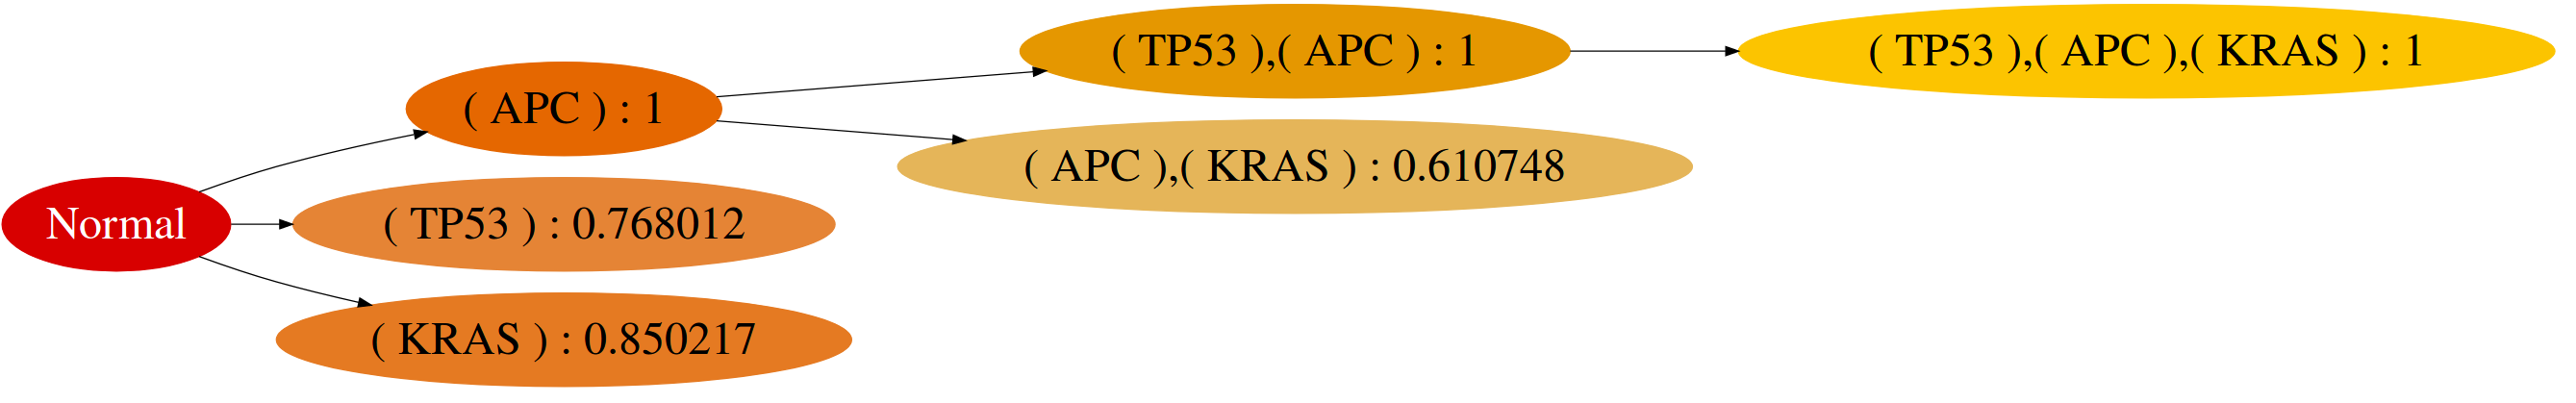
\includegraphics[scale=0.16, keepaspectratio]{COL_RESIC.png}% picture filename
	  \captionsetup{justification=centering,margin=0.5cm}
	  \caption{Colon retto $n.reseeds=1000$ $c=0.3$ (BML) Si può osservare come la mutazione sul gene APC preceda quella sul TP53 e come poi insieme favoriscano il sopraggiungere di una mutazione su KRAS} 
	\end{figure}

	\begin{figure}[H]
	  \centering
	  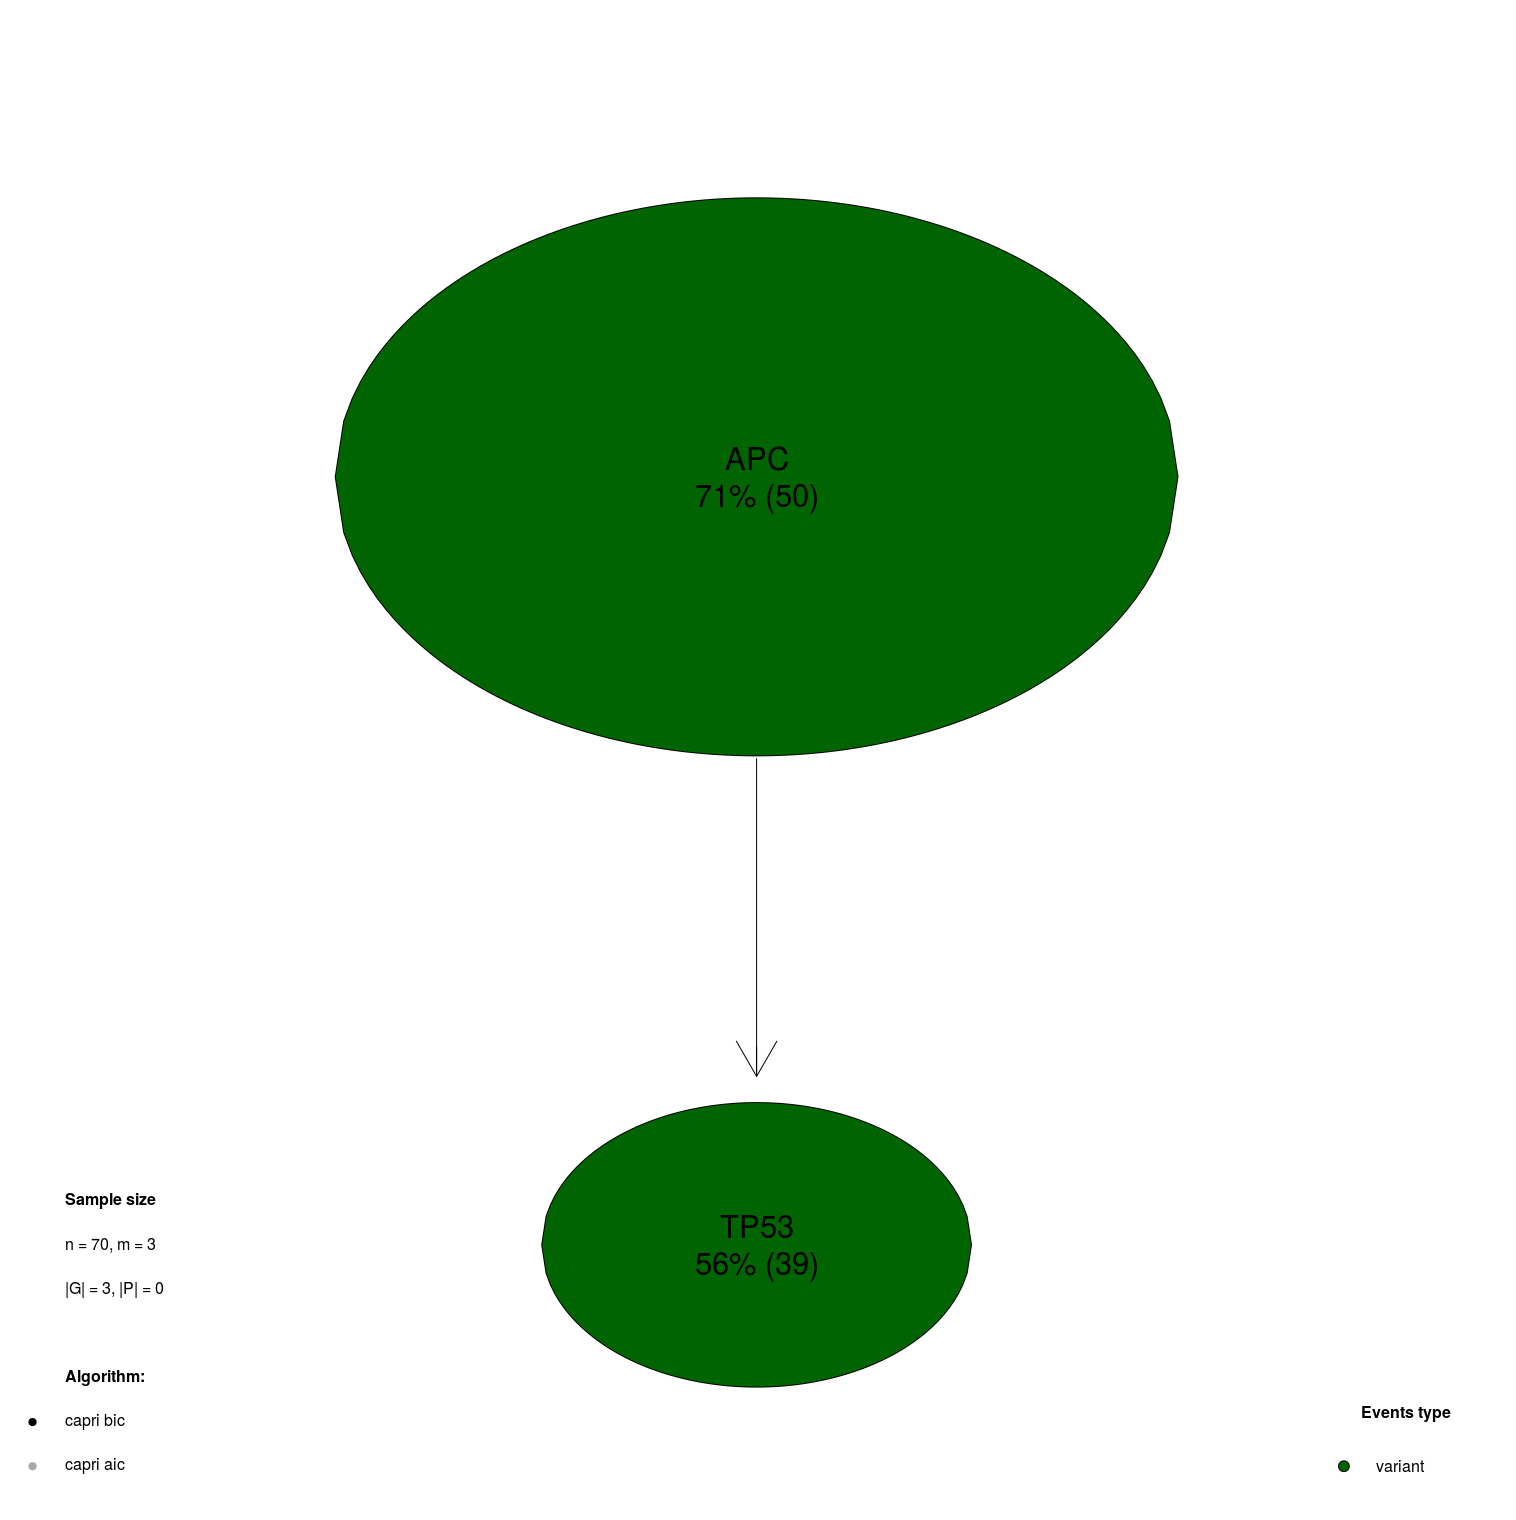
\includegraphics[height=12cm, keepaspectratio]{COL_RESIC_capri.png}% picture filename
	  \captionsetup{justification=centering,margin=0.5cm}
	  \caption{Tumore al Colon retto $n.boot=10000$ (CAPRI) I dati sono sufficienti a individuare solamente che APC precede TP53 (d'ora in poi ci riferiremo ai soli geni indicando mutazioni sul gene)}
	\end{figure}

	\begin{figure}[H]
	  \centering
	  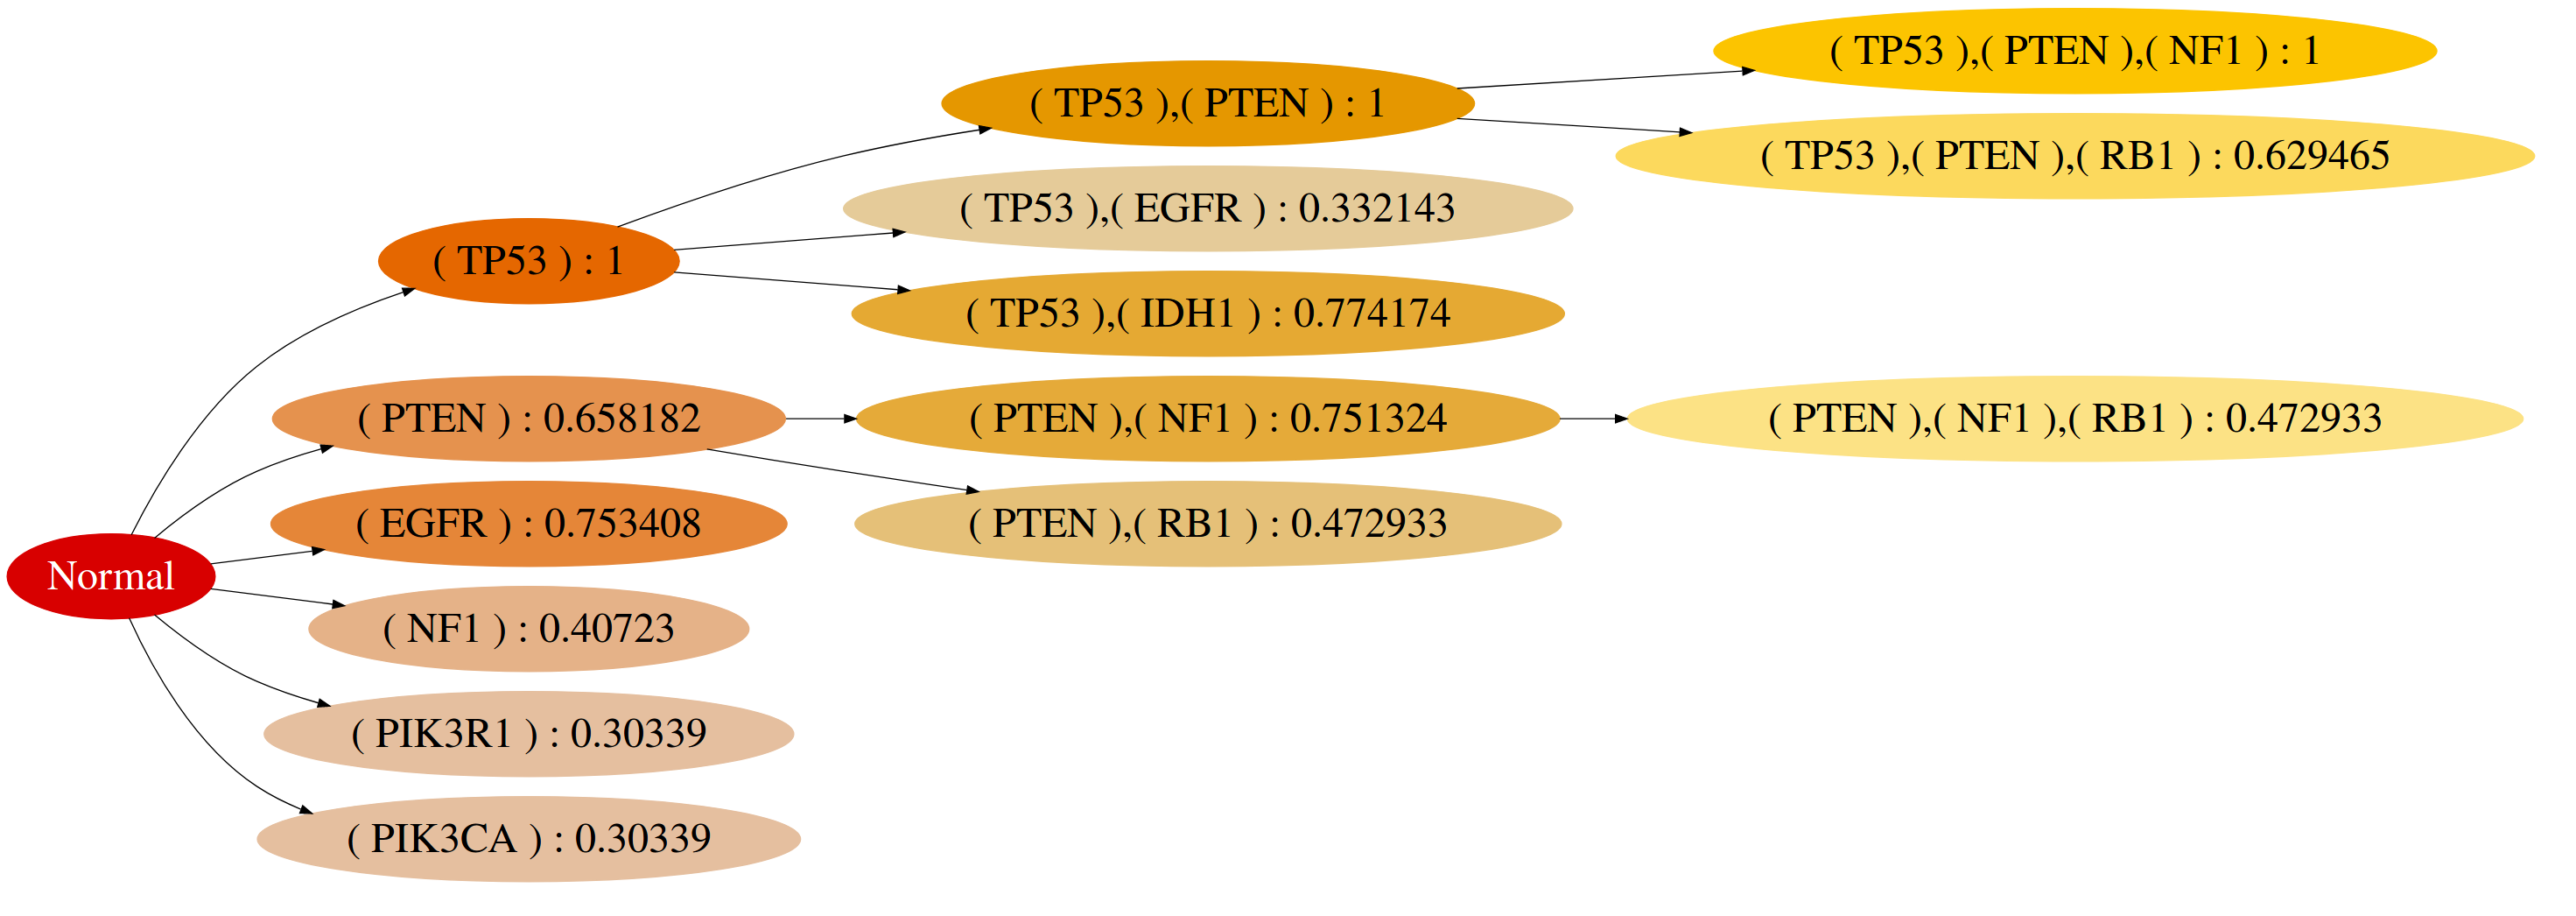
\includegraphics[height=5.5cm, keepaspectratio]{GBM_SM4.png}% picture filename
	  \captionsetup{justification=centering,margin=0.5cm}
	  \caption{Glioblastoma $n.reseeds=1000$ $c=0.3$ (BML) In questo caso grazie ad un dataset più ricco BML riconosce diversi percorsi evolutivi, viene inferito che TP53 favorisca PTEN caratteristica che non si
	            verifica su CAPRI (almeno con 1000 bootstrap resample). Per il resto si osservano invece comunque affinità fra i due risultati proposti } 
	\end{figure}

	\begin{figure}[H]
	  \centering
	  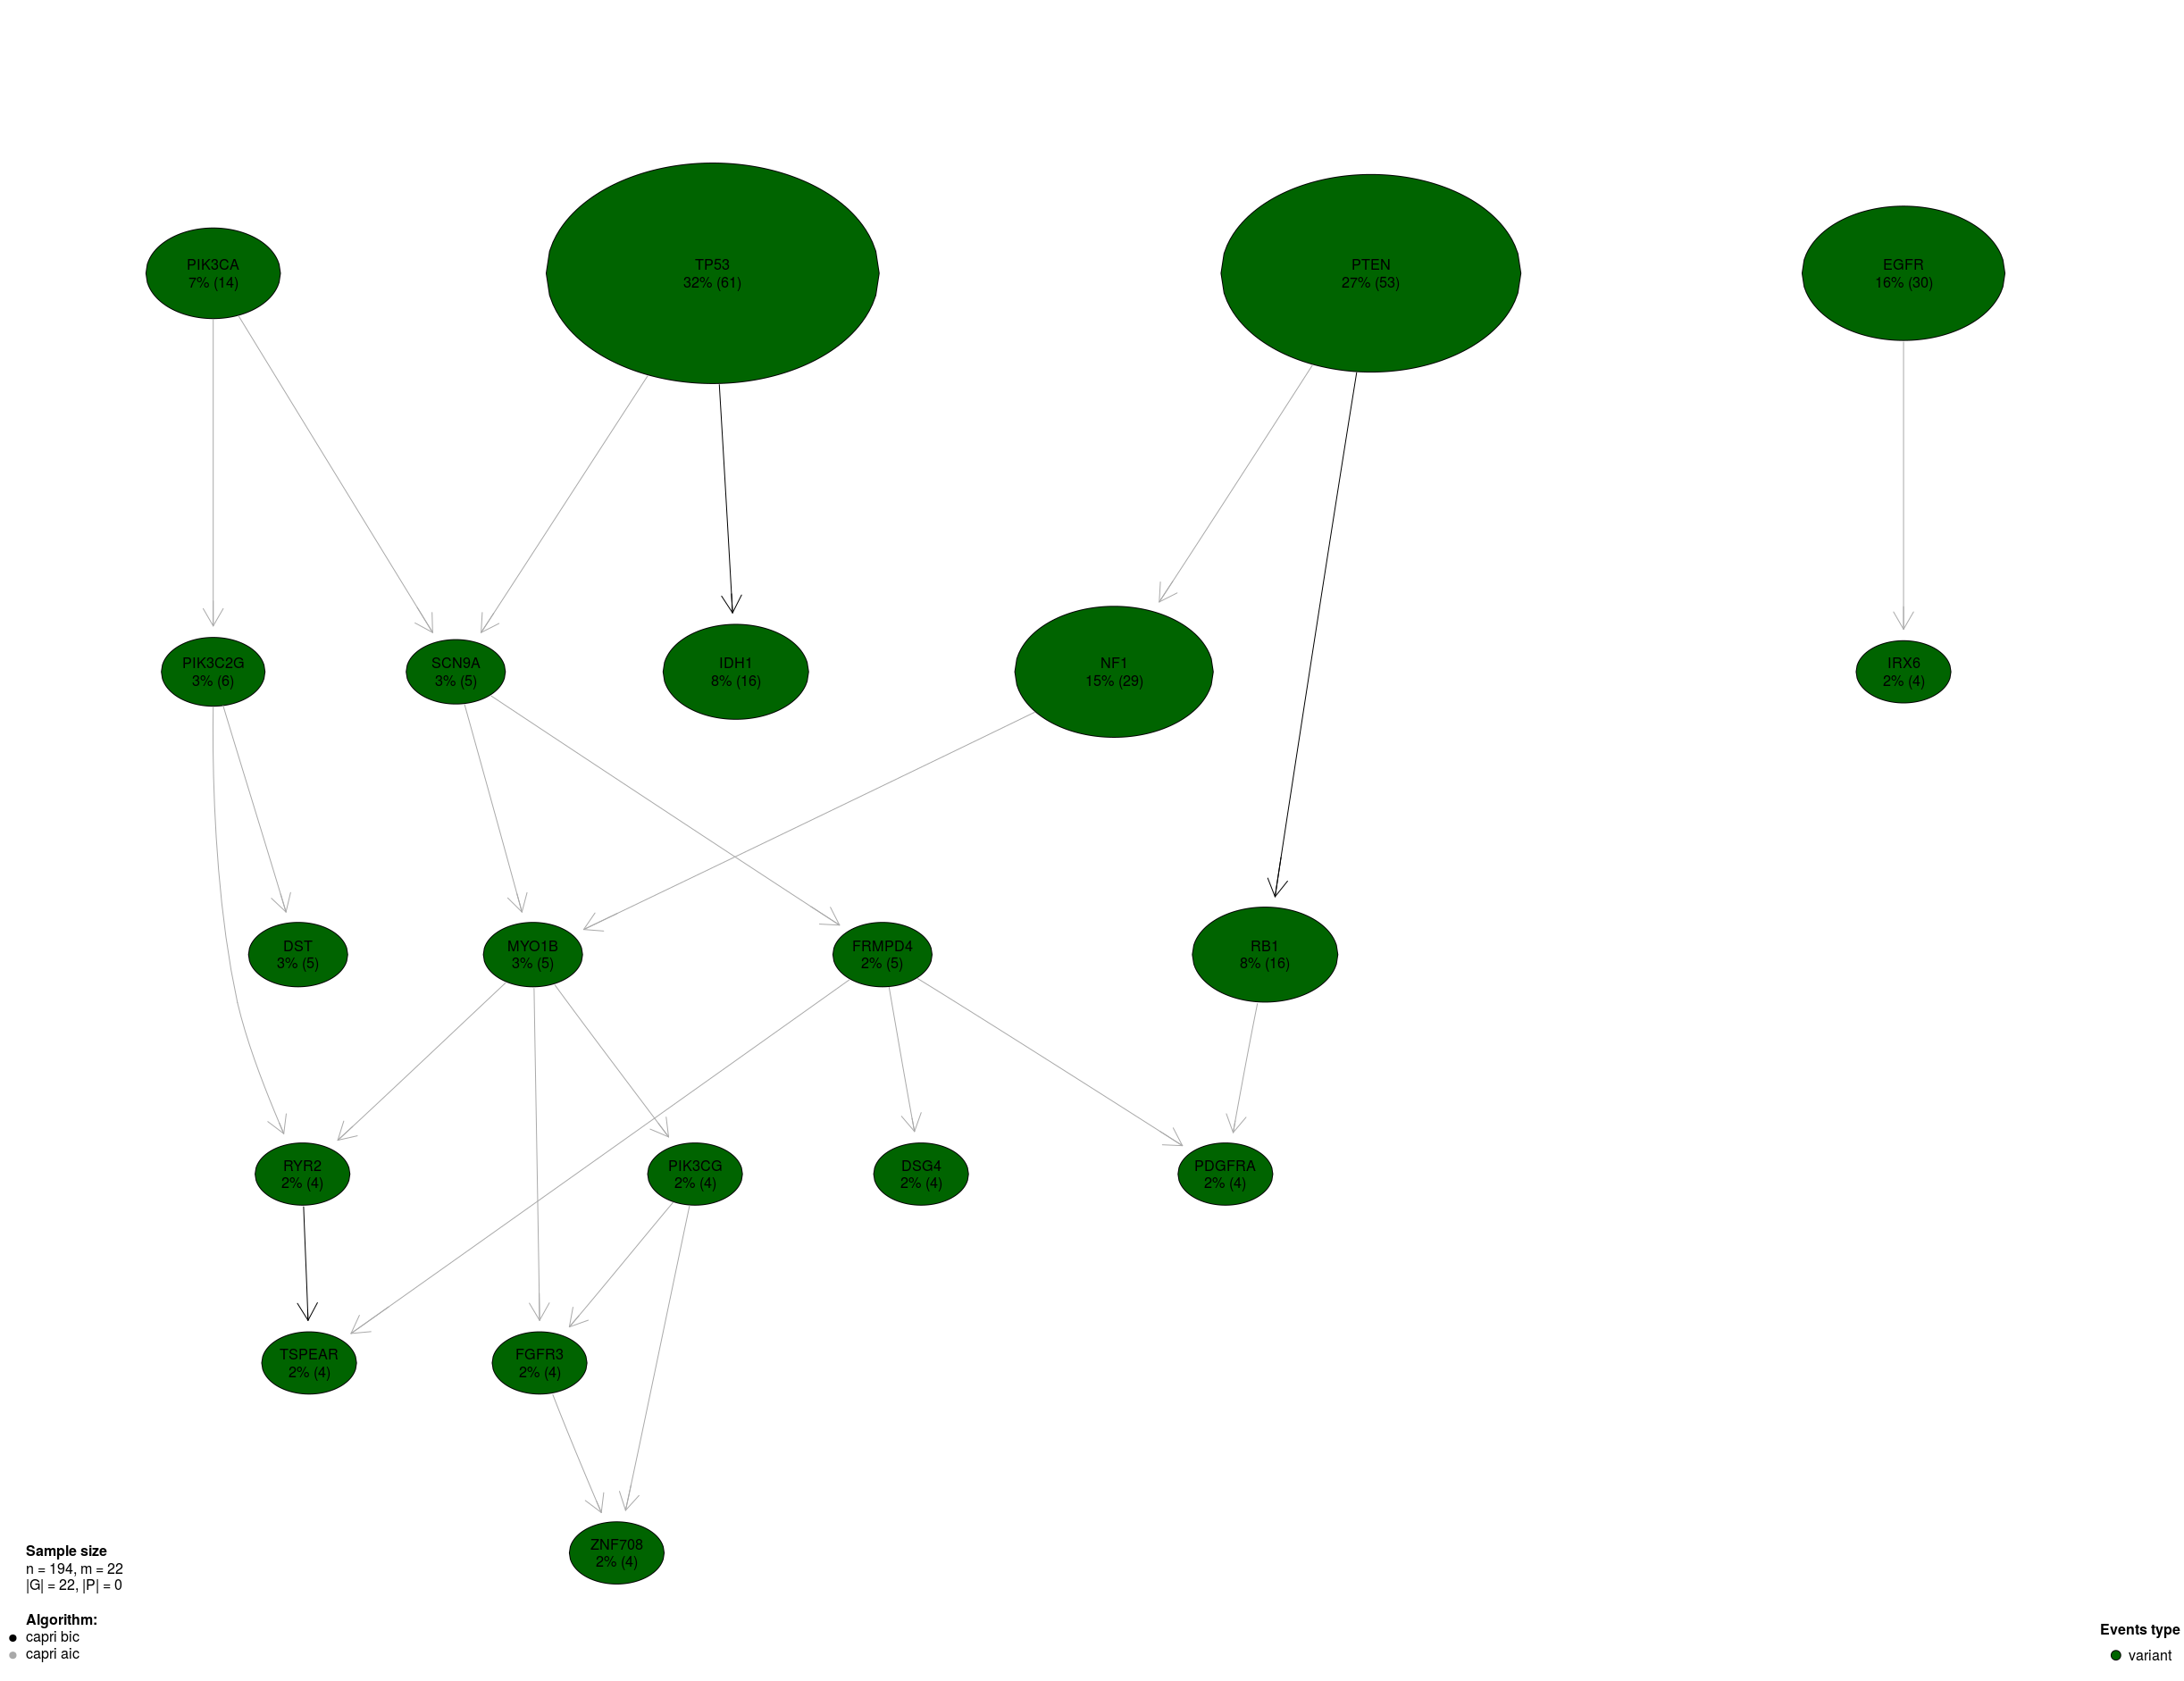
\includegraphics[height=12cm, keepaspectratio]{GBM_SM4_capri.png}% picture filename
	  \captionsetup{justification=centering,margin=0.5cm}
	  \caption{Glioblastoma $n.boot=1000$ (CAPRI), si osservi come diverse inferenze siano le stesse effettuate da BML (si tenga conto anche delle frecce grige sottili)} 
	\end{figure}

	\begin{figure}[H]
	  \centering
	  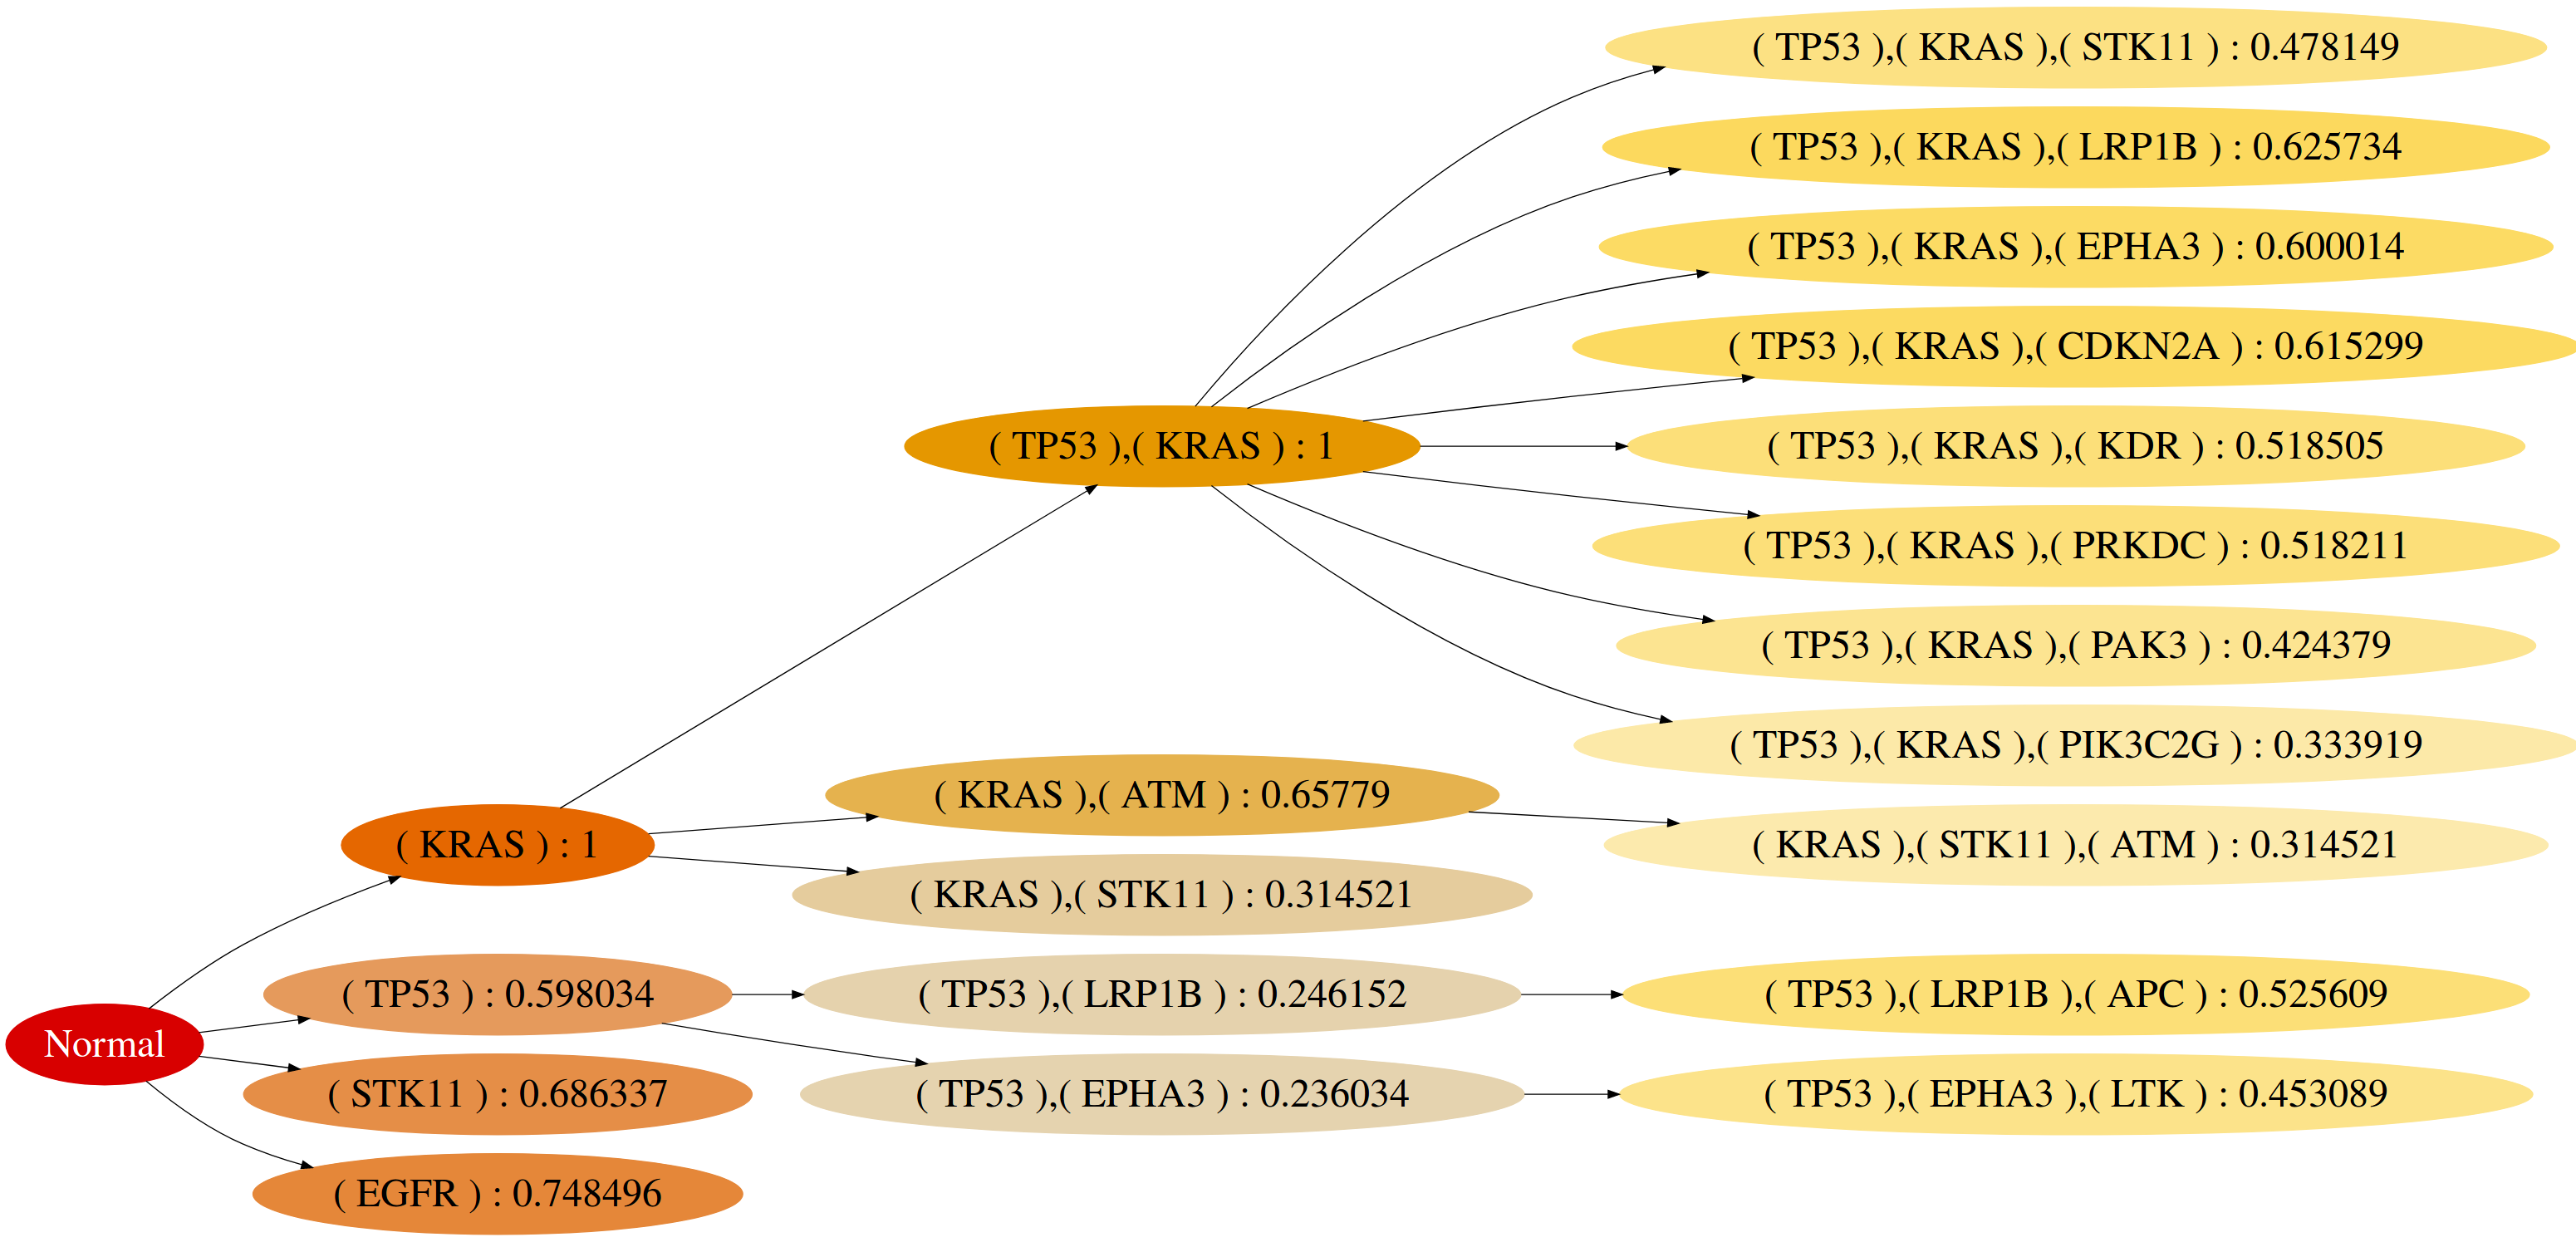
\includegraphics[height=7.5cm, keepaspectratio]{Lung_SM4.png}% picture filename
	  \captionsetup{justification=centering,margin=0.5cm}
	  \caption{Tumore ai polmoni $n.reseeds=1000$ $c=0.3$ (BML) Anche in questo caso i due risultati sono comparabili} 
	\end{figure}

	\begin{figure}[H]
	  \centering
	  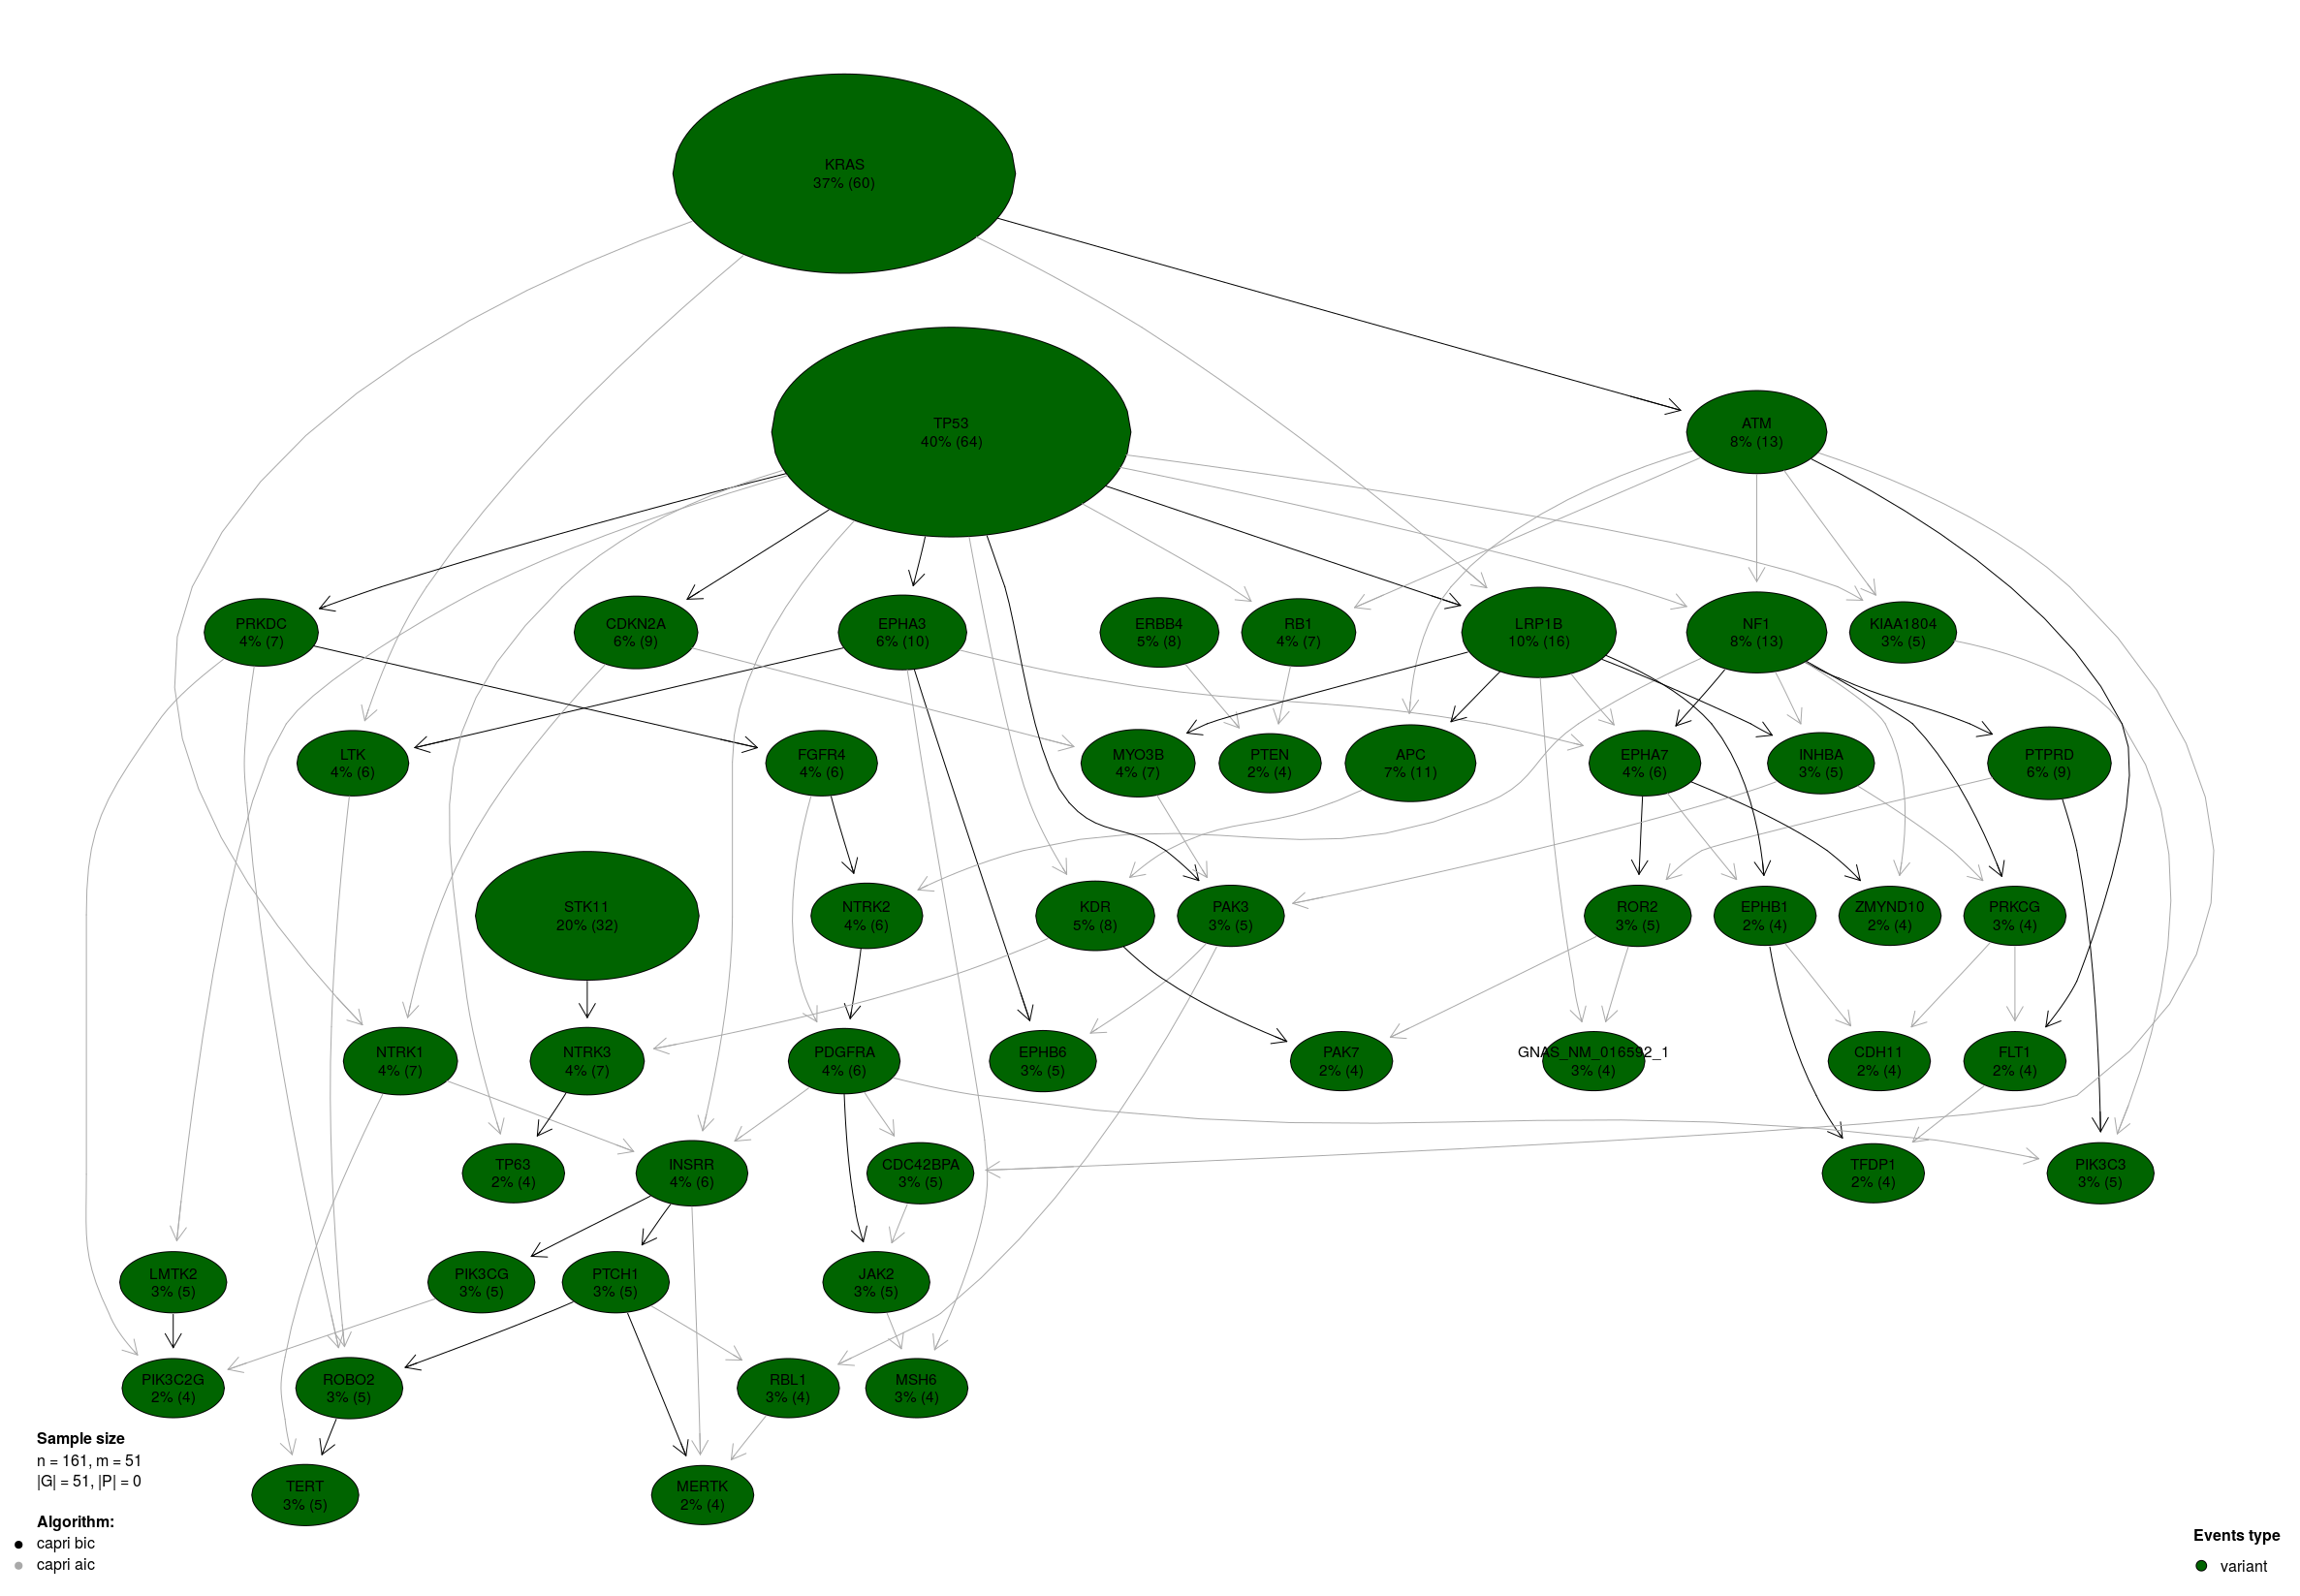
\includegraphics[height=11cm, keepaspectratio]{Lung_SM4_capri.png}% picture filename
	  \captionsetup{justification=centering,margin=0.5cm}
	  \caption{Tumore ai polmoni $n.boot=1000$ (CAPRI) Per verificare se la relazione KRAS-TP53 fosse inferita anche da CAPRI si è effettuata l'analisi anche con 10000 ricampionamenti
			(richiedendo poco più di un'ora di elaborazione)} 
	\end{figure}

	\begin{figure}[H]
	  \centering
	  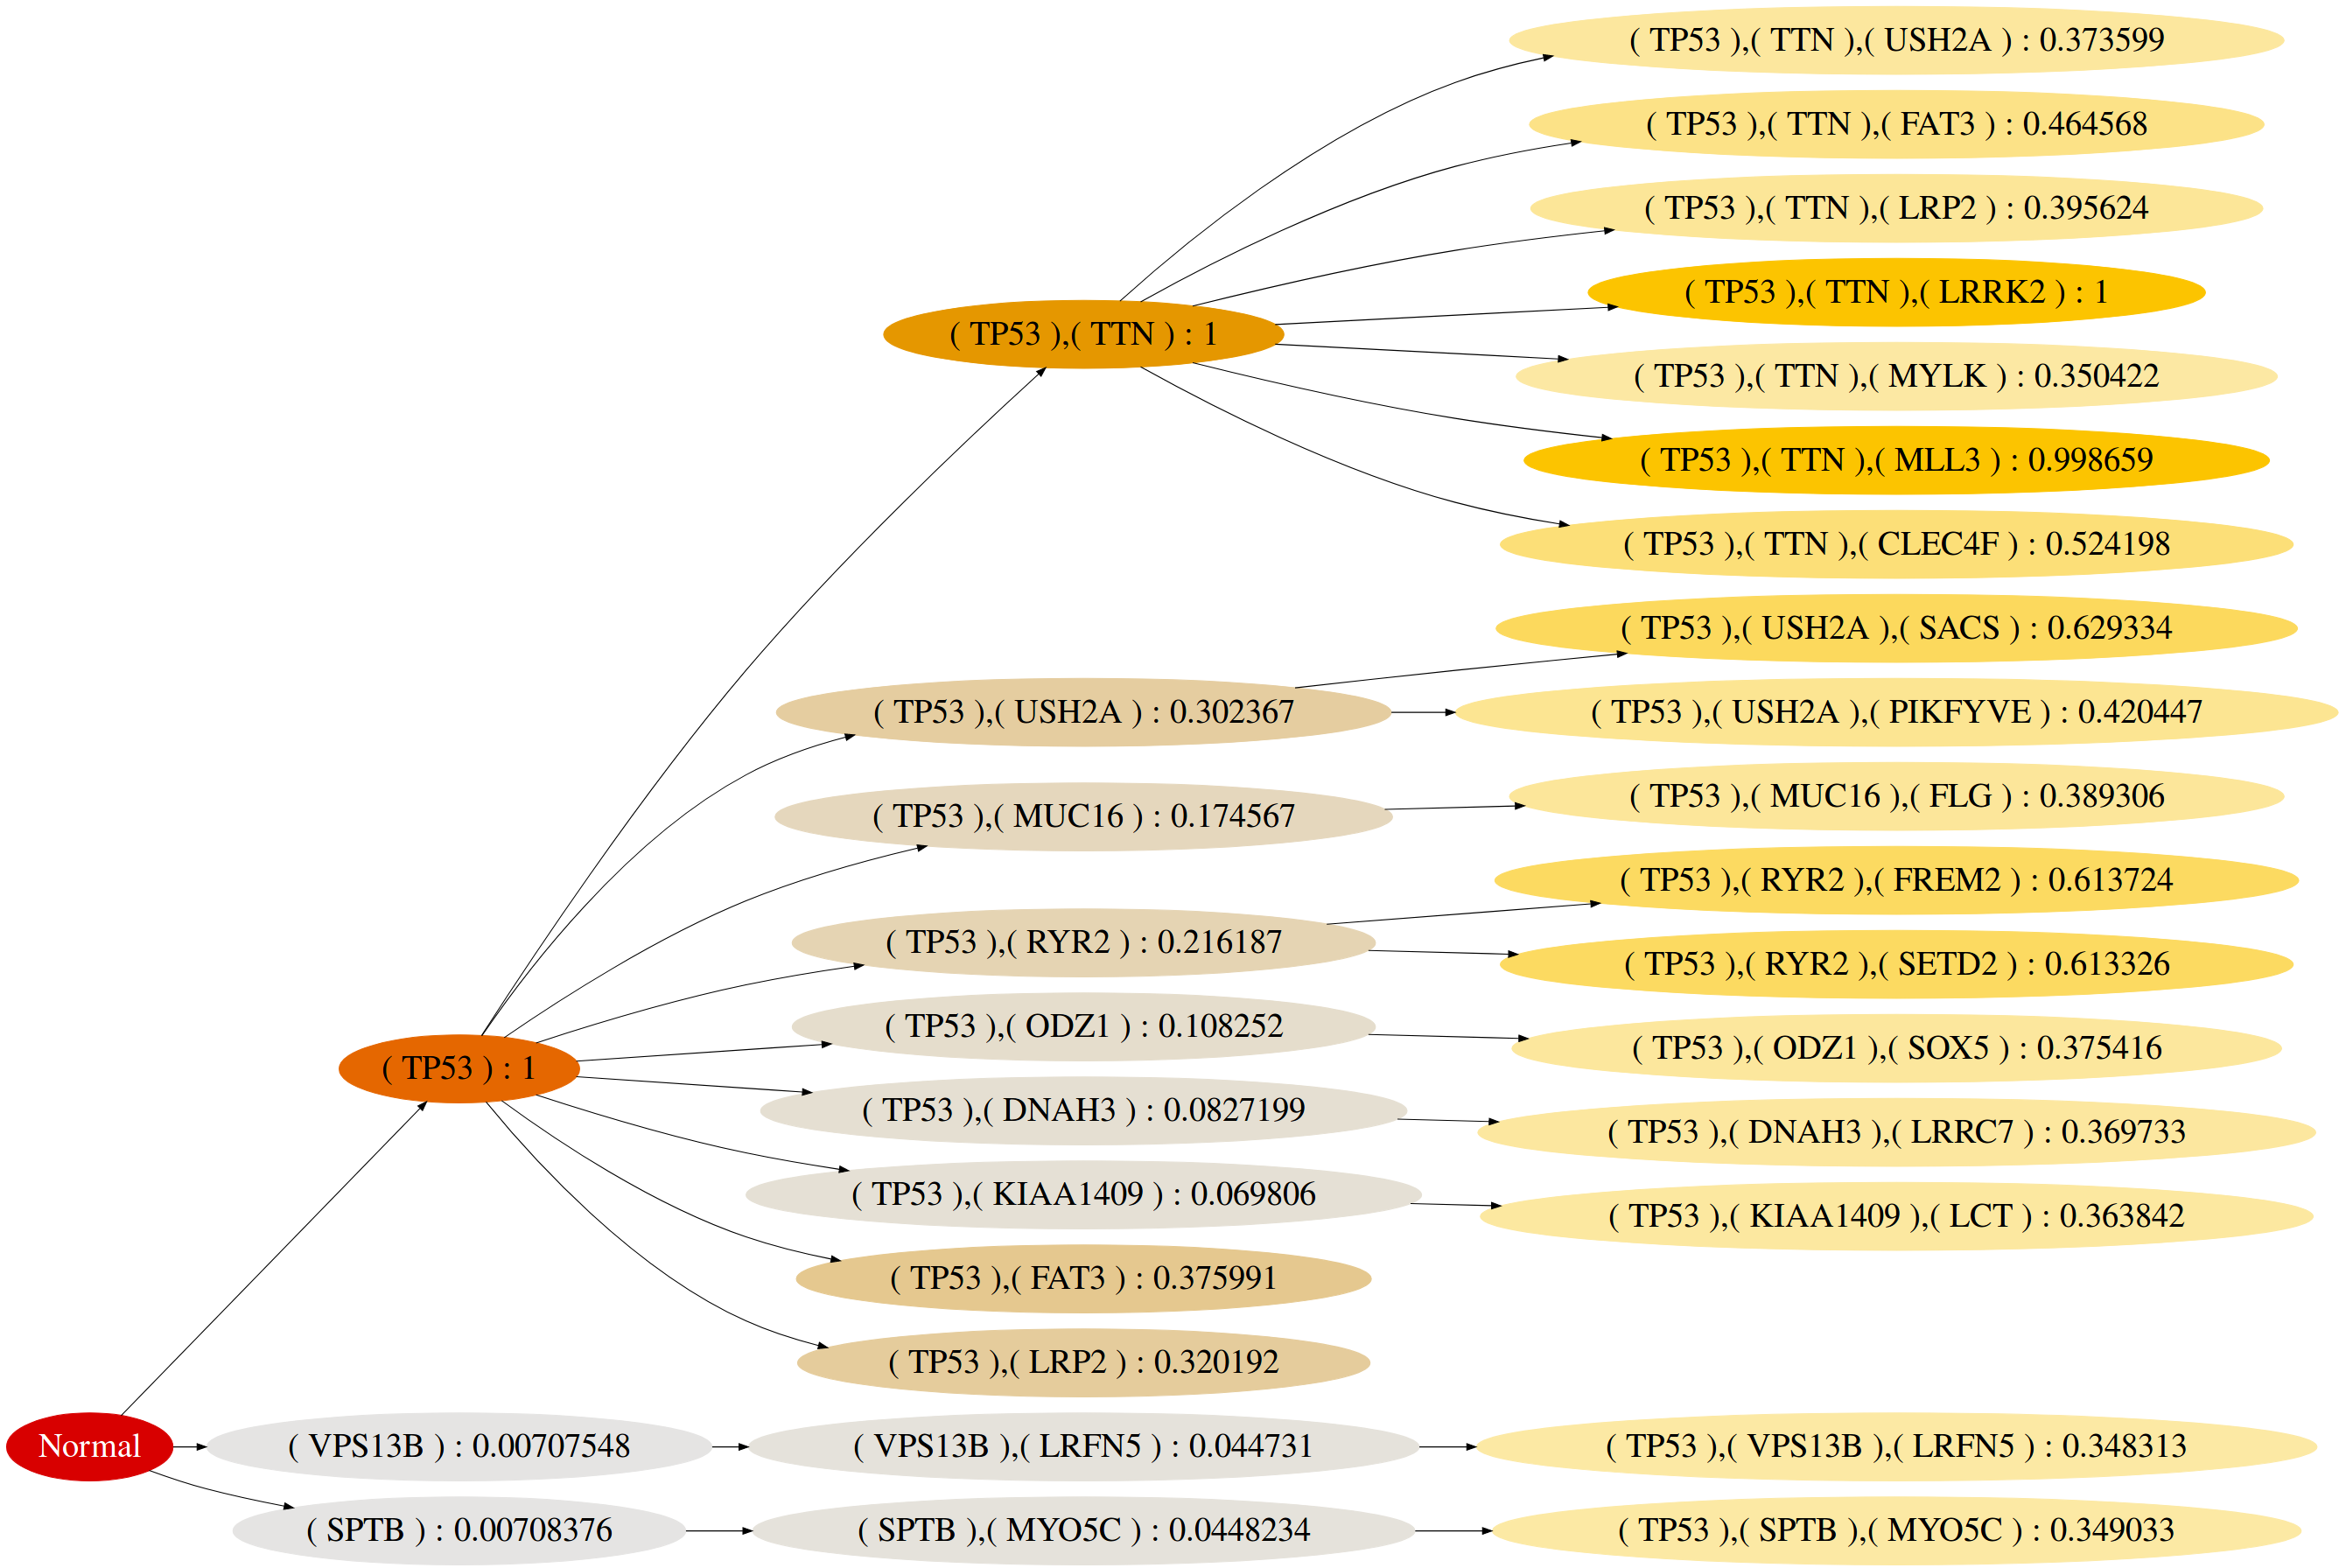
\includegraphics[height=8.5cm, keepaspectratio]{OV_SM5.png}% picture filename
	  \captionsetup{justification=centering,margin=0.5cm}
	  \caption{Tumore alle ovaie $n.reseeds=100$ $c=0.3$ (BML) I dati di questo studio coinvolge un numero di geni che rende la visualizzazione dei grafi di CAPRI difficile,
	 	   comunque vi è un sostanziale accordo} 
	\end{figure}

	\begin{figure}[H]
	  \centering
	  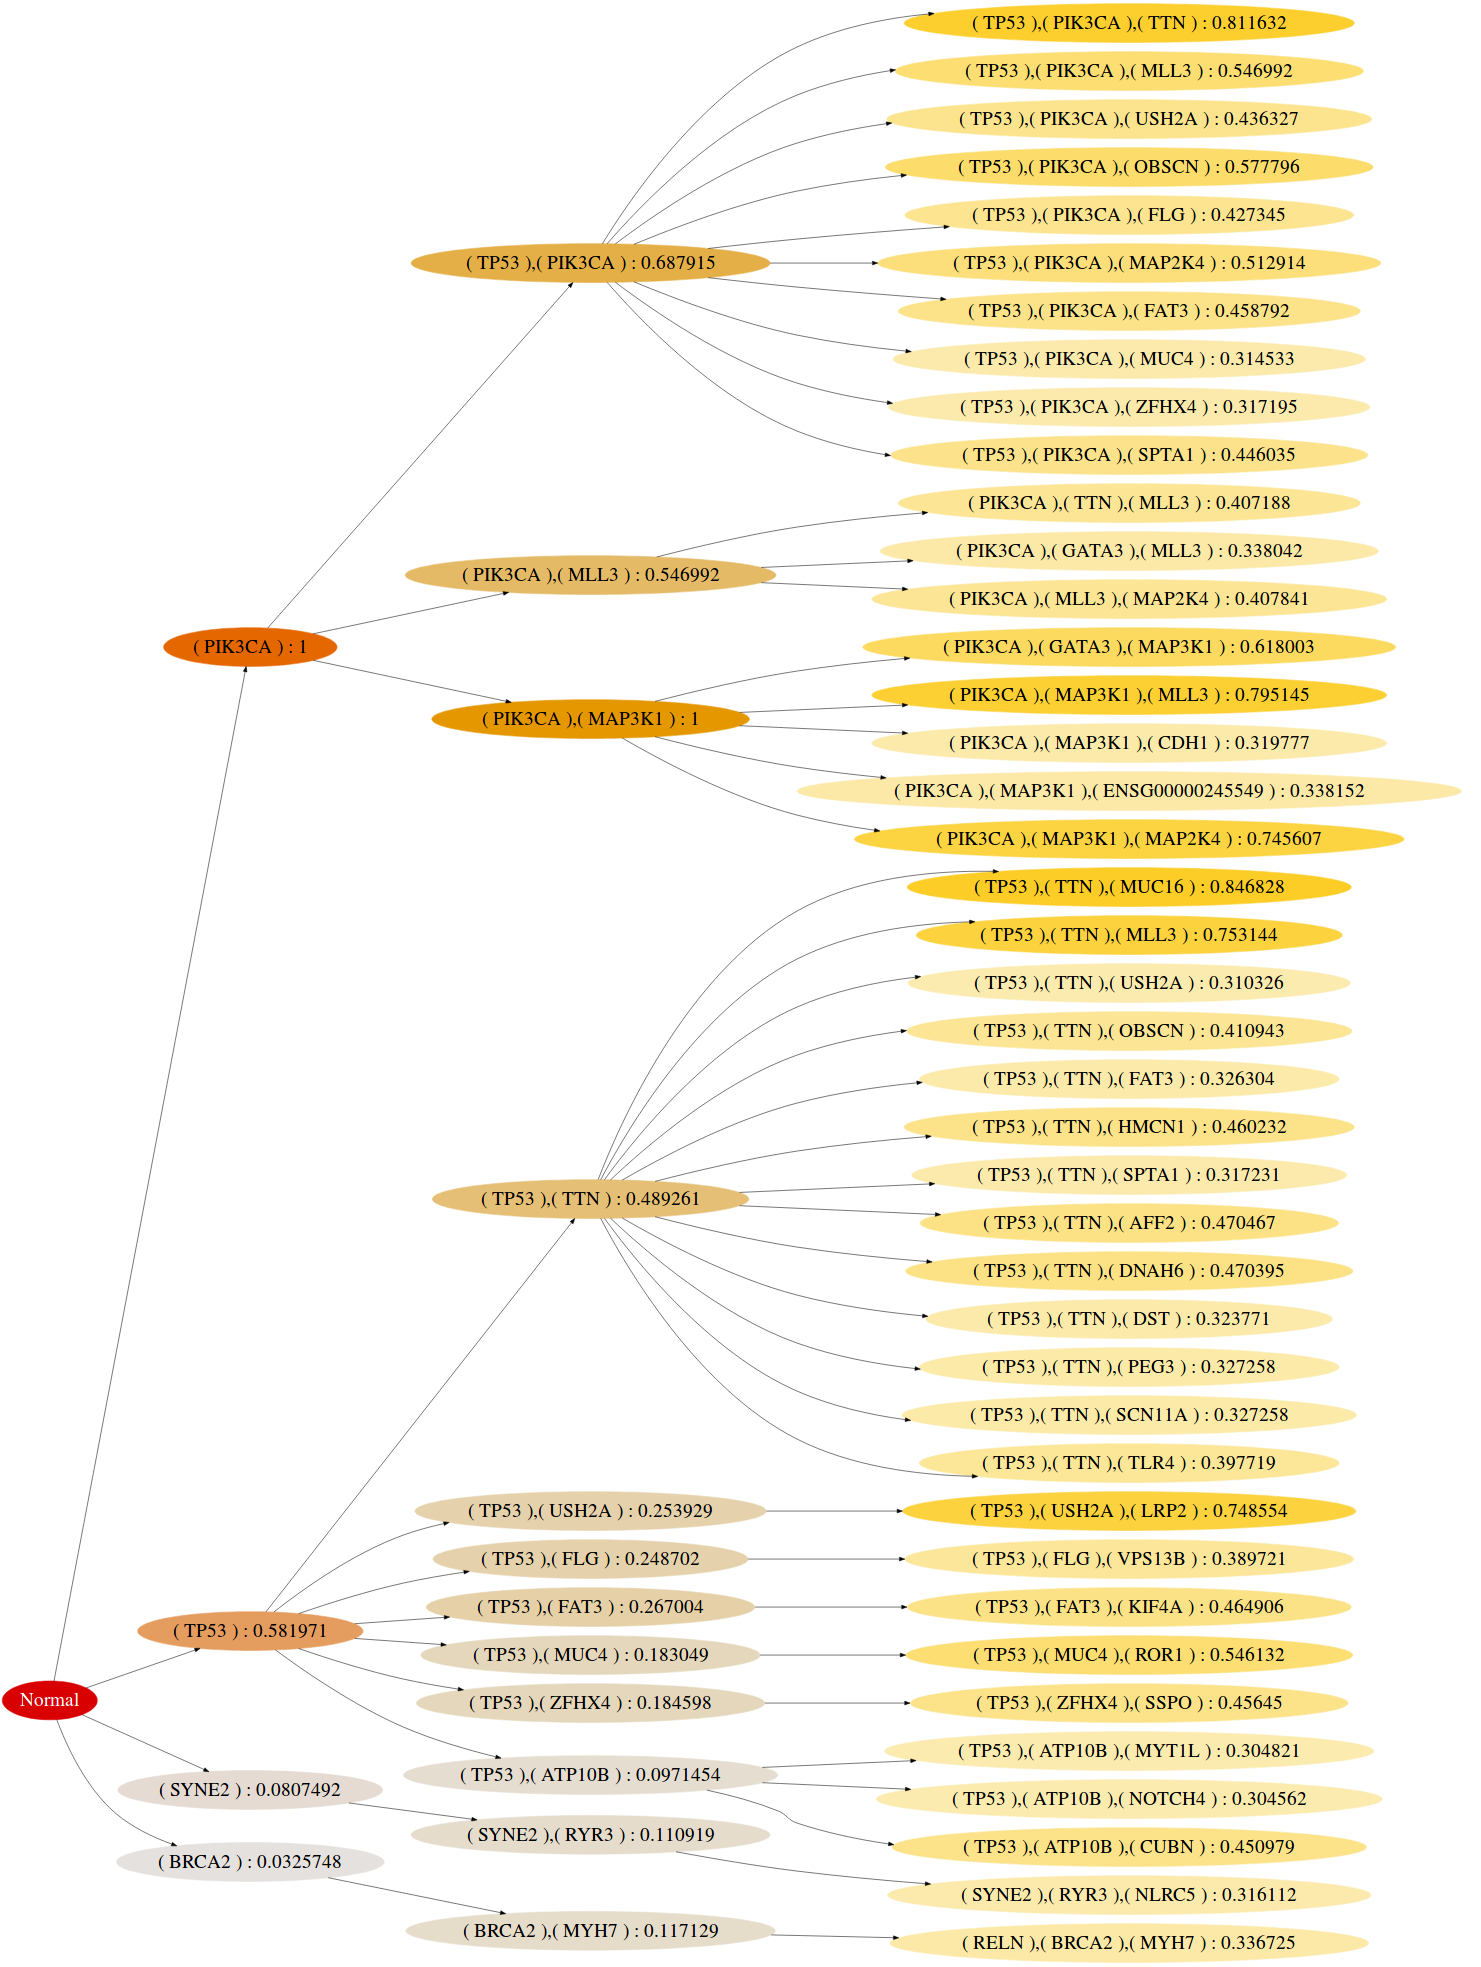
\includegraphics[height=11cm, keepaspectratio]{BRCA_SM7.png}% picture filename
	  \captionsetup{justification=centering,margin=0.5cm}
	  \caption{Tumore al seno $n.reseeds=100$ $c=0.3$ (BML) Anche in questo studio (ancora più ricco di dati) si osserva compatibilità almeno fra le relazioni principali, si ricorda che BML scarta molte relazioni a bassa probabilità} 
	\end{figure}

	\begin{figure}[H]
	  \centering
	  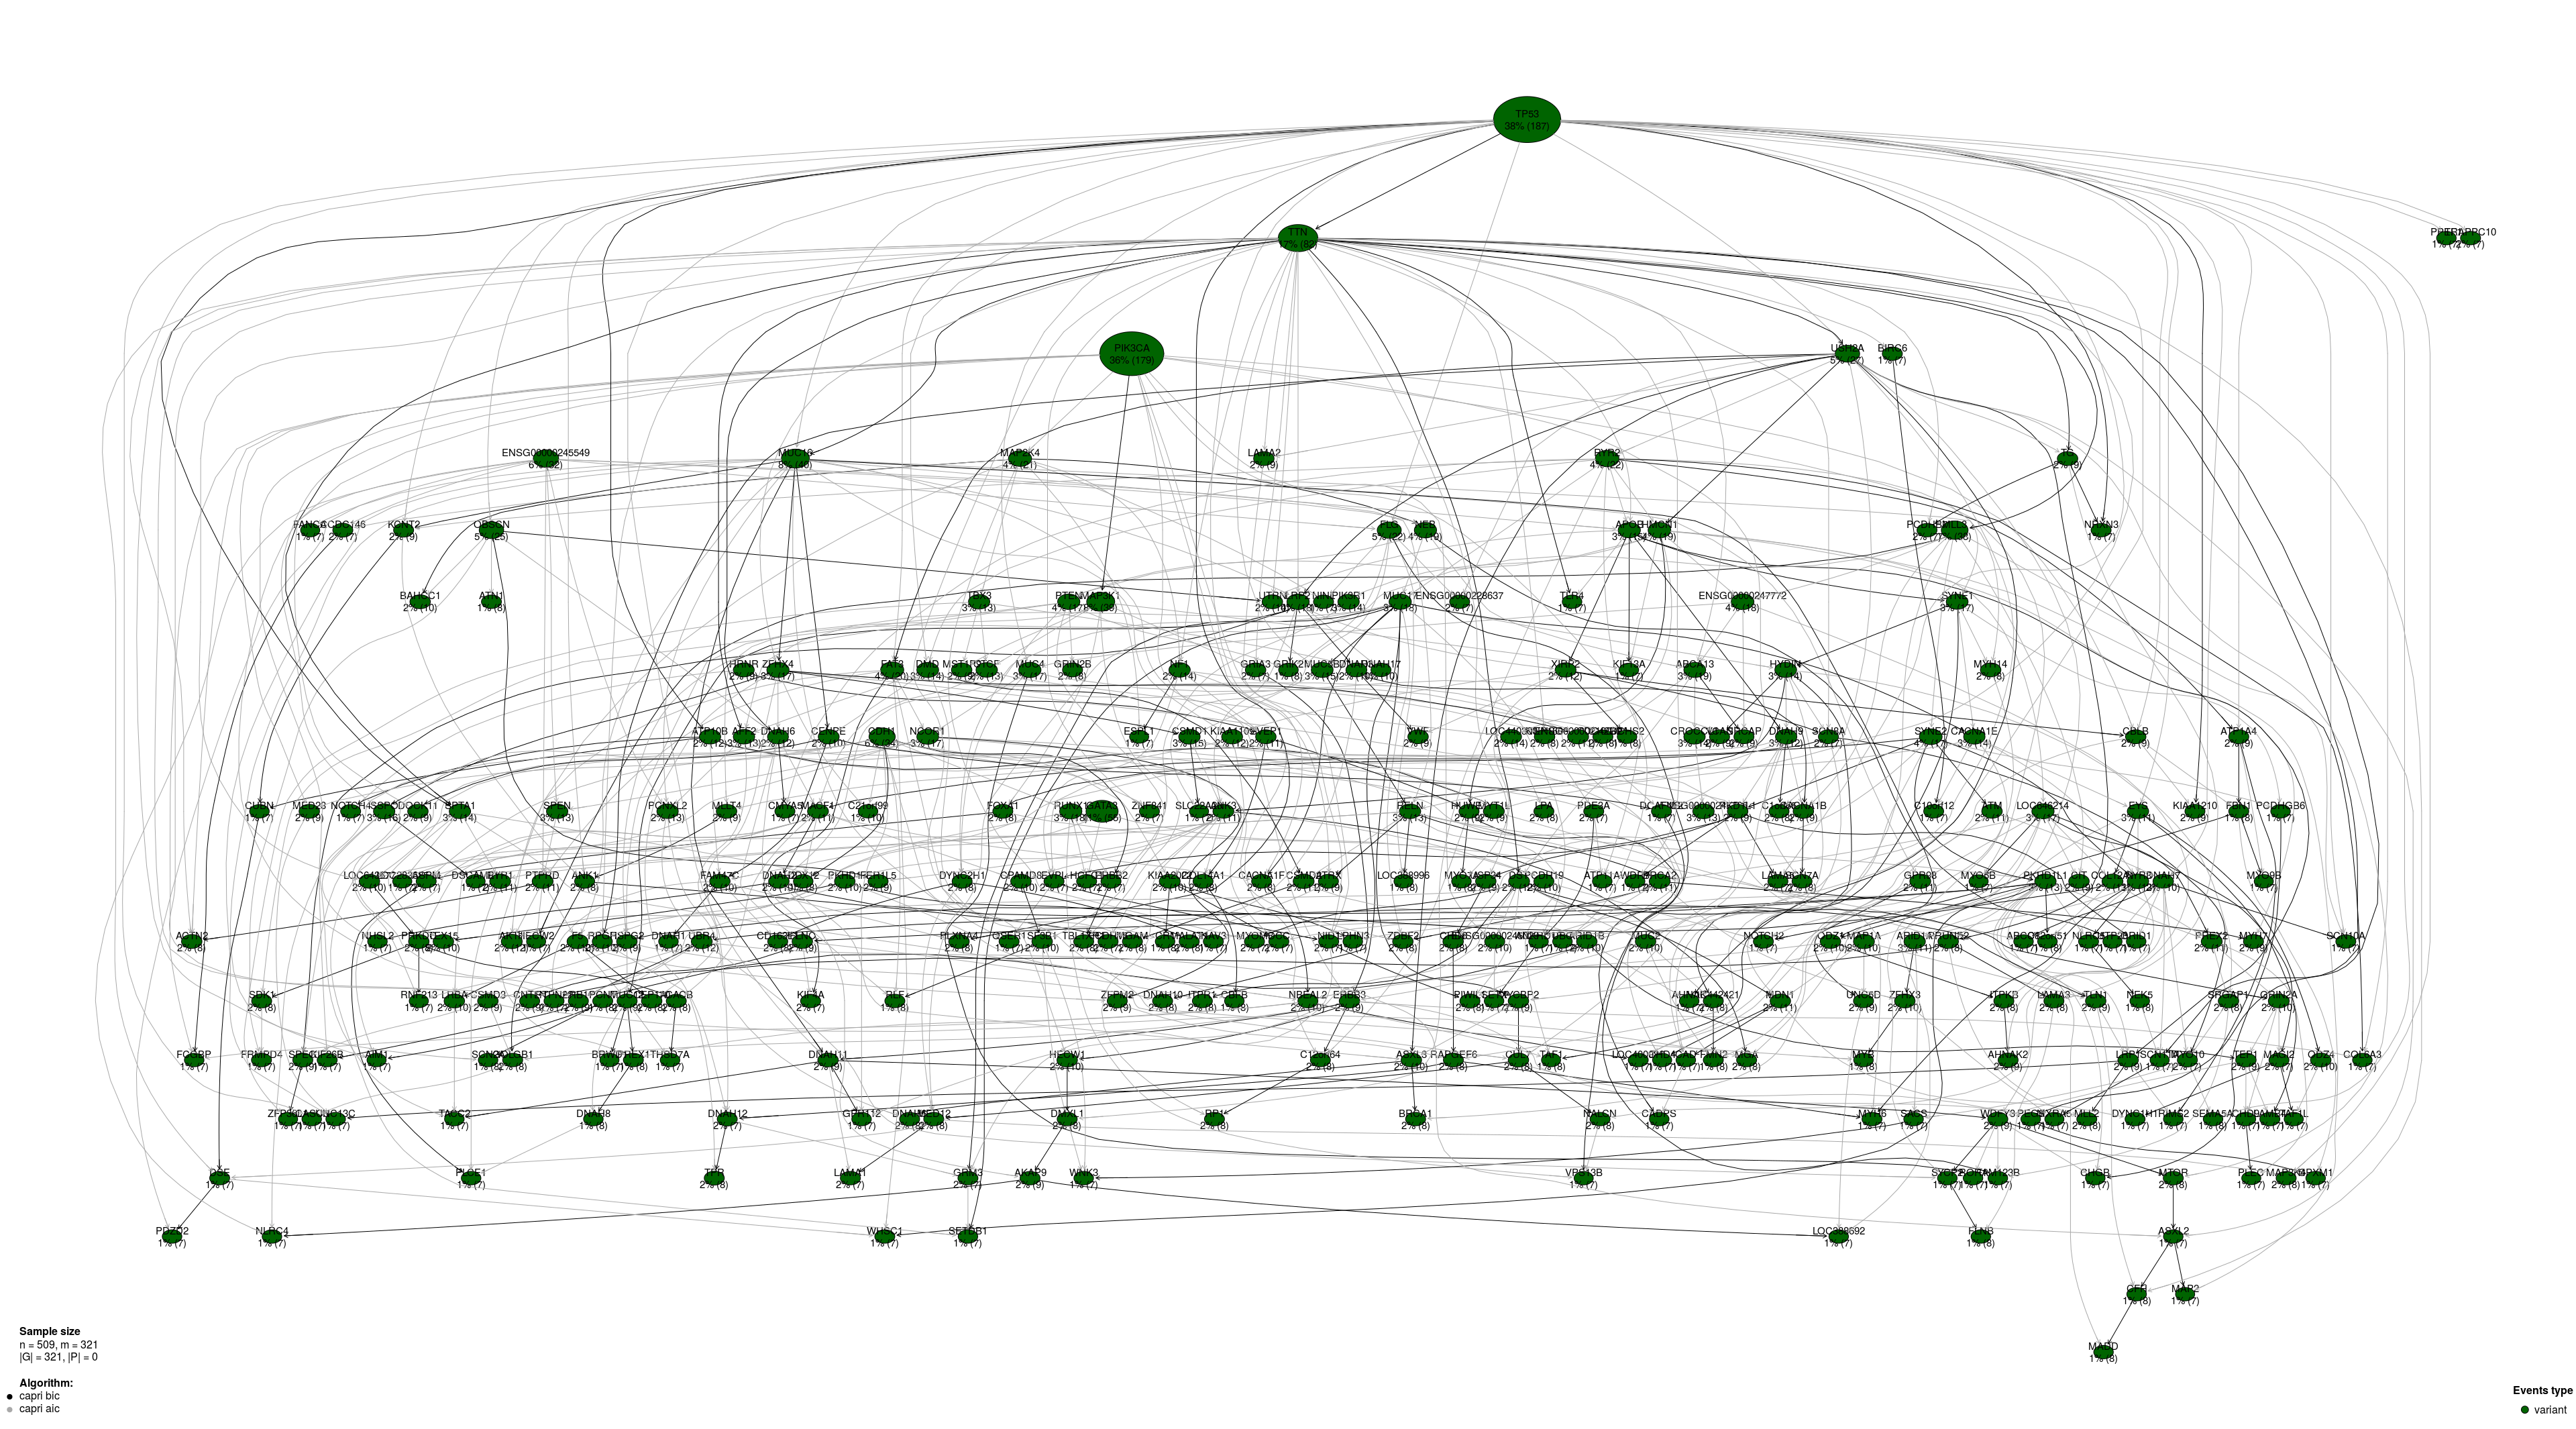
\includegraphics[height=8cm, keepaspectratio]{BRCA_SM7_capri.png}% picture filename
	  \captionsetup{justification=centering,margin=0.5cm}
	  \caption{Tumore al seno $n.boot=30$ (CAPRI), come si può vedere il grafo non è facilmente interpretabile e visualizzabile se non su schermi ad alta risoluzione} 
	\end{figure}

	Non è possibile al momento fare delle considerazioni specifiche su quale dei due metodi sia più accurato e sarebbe necessario produrre un insieme
	sostanzioso di dataset artificiali che evidenzino con precisione le differenze fra i due metodi. Per essere efficaci queste simulazioni dovrebbero 
	considerare come si possa normalmente evolvere un cancro basandosi sulle teorie attuali e cercando al più possibile di replicarle, permettendo 
	così di creare della casistica operativa di senso compiuto.

	\subsection{\large Note sul lavoro di Alice Tarzariol}	
	
	La studentessa Alice Tarzariol ha realizzato recentemente un programma per lo studio dei percorsi evolutivi nel cancro (Mutation Evolution Analyzer \cite{Alice})
	sfruttando non solo le mutazioni ma anche le informazioni temporali relative ad uno specifico studio. 
	Data la specificità del software così preparato è impossibile confrontarlo con BML dato che quest'ultimo non 
	prevede che nei suoi input ci possano essere degli stadi intermedi del tumore. E' invece possibile analizzare gli 
	stessi dati tramite CAPRI, ma i risultati non sono comparabili e frequentemente sono in disaccordo. Sarebbe inoltre necessario 
	trovare un altro studio che fornisca dati temporali sulle mutazioni osservate per testare più approfonditamente questo programma.
	Segnalo inoltre un minore contributo personale volto alla riorganizzazione del codice (e correzione di alcuni errori minori) 
	per l'applicazione Java che ne permette l'uso (scaricabile da qui \cite{AliceNew}). 	
	  	 
	\section{\LARGE Conclusione}	

	Dai risultati ottenuti appare sufficientemente chiaro come BML e CAPRI siano almeno in parte comparabili e come il loro comportamento 
	tenda ad assomigliarsi. Ciò nonostante è necessario effettuare più test su casistica specifica per entrambi i software, 
	prendendo in considerazione nuovi studi ed adattandoli per l'analisi. Inoltre è essenziale introdurre differenti metodologie 
	e modelli nella comparazione, per verificare che le similitudini non siano esclusivamente dovute a quelle del modello 
	che BML e CAPRI usano. 

	Per concludere presentiamo le problematiche ancora aperte nel campo della filogenetica dei tumori, come sono state illustrate nella review di Science di cui si
	è discusso precedentemente. 

	\begin{itemize}
	\item \textbf{Sfruttare multipli o nuovi marker}: La maggior parte delle metodologie considera CNV e/o SNV con alcune eccezioni (come CAPRI) che si 
	adattano a metilazione o marker istonici. Non vi sono sistemi che cerchino di integrare le informazioni e che riescano a considerare alcuni 
	segnali, come ad esempio la distribuzione cellulare nel tumore.	
	\item \textbf{Modelli generali}: Non sono ancora disponibili dei modelli adatti a spiegare il comportamento di fenomeni complessi come cromoplexis e katageis
	e dei modelli che si adattino specificatamente a situazioni particolari e tengano conto di più parametri, come il livello di selezione, dello specifico paziente e
	il tempo di mutazione.
	\item \textbf{Algoritmi specifici per i tumori}: la maggior parte degli algoritmi utilizzati finora sfrutta dei metodi di inferenza che si basano sull'analisi
	filogenetica delle specie e non è chiaro se questi possono essere adatti all'analisi dei tumori. E' necessario approfondire quindi questo argomento 
	tenendo conto di comportamenti differenti.  
	\item \textbf{Superare gli alberi delle specie}: I modelli basati su alberi potrebbero non essere adeguati alla spiegazione dei processi evolutivi di 
	tutti i tipi di cancro in quanto spesso si verificano situazioni di co-esistenza di diverse subpopolazioni clonali e presumibilmente quindi di co-evoluzione.
	Solo ora si stanno iniziando a sviluppare sistemi che tengano conto anche di questo.
	\item \textbf{Analisi statistica e riproducibilità}: E' necessario rendere sistematiche e ripetibili le analisi effettuate in questo settore. 
	Nello specifico è necessario riuscire ad avere una sufficiente quantità di dati, che spesso è carente almeno nelle analisi single cell, e 
	cercare di creare degli studi che si focalizzino su questo scopo direttamente e non come secondo fine. 
	\end{itemize}
		
	In questo lavoro abbiamo quindi considerato dapprima un testo introduttivo che illustra il mondo dell'analisi filogenetica dei tumori, successivamente 
	abbiamo approfondito il funzionamento di
	un programma atto a questo scopo, le modifiche a lui realizzate e una metodologia alternativa ed infine comparato le due soluzioni 
	individuando similitudini nel risultato ottenuto. 

	%---------------------- BIBLIOGRAFIA

	\begin{thebibliography}{20}

	\bibitem{Nowell}
	   Nowell, The clonal evolution of tumor cell populations, Science 194, 23-28 (1976)
	\bibitem{Review}
	   Schwartz R. et al., The evolution of tumor phylogenetics: principles and practice, Science Review, 213-229 (2017)
	\bibitem{BMLPub}
	   Misra N. et al., Inferring the paths of somatic evolution in cancer, Oxford University Press Bioinformatics Vol. 30 no. 17 2014, pages 2456-2463
        \bibitem{BFBImage}
           Samuel F. Bunting and Andre Nussenzweig, End-joining, translocations and cancer, Nature Reviews Cancer 13, 443–454 (2013)
	\bibitem{Tsao}
		Tsao J et al., Tracing cells fates in human colorectal tumors from somatic microsatellite mutations: evidence of adenomas with stem cell architecture,
		Am. J. Pathol, 153, 1189-1200 (1998)
	\bibitem{Desper}
		Desper R. et al, Inferring tree models of oncogenetics from comparative genomic hybridization data, 6, 37-51 (1999)
	\bibitem{FerVog}
		Fearon E. and Vogelstein B., A genetic model for colorectal tumorigenesis, Cell 61, 759-767 (1990)
	\bibitem{MAF}
		https://wiki.nci.nih.gov/display/TCGA/Mutation+Annotation+Format+(MAF)+Specification
	\bibitem{cBio}
		http://www.cbioportal.org/
	\bibitem{BMLSite}
		http://bml.molgen.mpg.de/
	\bibitem{Qt}
		http://TODO
	\bibitem{TRONCO}
		De Sano L. et al., TRONCO: an R package for the inference of cancer progression models from heterogeneous genomic data, arXiv:1509.07304  [q-bio.QM] (2015)
	\bibitem{CAPRI}
		Ramazzotti et al., CAPRI: efficient inference of cancer progression models from cross-sectional data, Bioinformatics, 31(18) (2015)
	\bibitem{Alice}
		Tarzariol A., Towards a Logic Programming tool for cancer analysis
	\bibitem{AliceNew}
		http://TODO
		
        \end{thebibliography}

\end{document}



